\documentclass[12pt,]{article}
\usepackage{lmodern}
\usepackage{amssymb,amsmath}
\usepackage{ifxetex,ifluatex}
\usepackage{fixltx2e} % provides \textsubscript
\ifnum 0\ifxetex 1\fi\ifluatex 1\fi=0 % if pdftex
  \usepackage[T1]{fontenc}
  \usepackage[utf8]{inputenc}
\else % if luatex or xelatex
  \ifxetex
    \usepackage{mathspec}
  \else
    \usepackage{fontspec}
  \fi
  \defaultfontfeatures{Ligatures=TeX,Scale=MatchLowercase}
\fi
% use upquote if available, for straight quotes in verbatim environments
\IfFileExists{upquote.sty}{\usepackage{upquote}}{}
% use microtype if available
\IfFileExists{microtype.sty}{%
\usepackage{microtype}
\UseMicrotypeSet[protrusion]{basicmath} % disable protrusion for tt fonts
}{}
\usepackage[margin=1in]{geometry}
\usepackage{hyperref}
\PassOptionsToPackage{usenames,dvipsnames}{color} % color is loaded by hyperref
\hypersetup{unicode=true,
            pdftitle={Draft},
            pdfauthor={Tim Radtke},
            colorlinks=true,
            linkcolor=Maroon,
            citecolor=Blue,
            urlcolor=blue,
            breaklinks=true}
\urlstyle{same}  % don't use monospace font for urls
\usepackage{graphicx,grffile}
\makeatletter
\def\maxwidth{\ifdim\Gin@nat@width>\linewidth\linewidth\else\Gin@nat@width\fi}
\def\maxheight{\ifdim\Gin@nat@height>\textheight\textheight\else\Gin@nat@height\fi}
\makeatother
% Scale images if necessary, so that they will not overflow the page
% margins by default, and it is still possible to overwrite the defaults
% using explicit options in \includegraphics[width, height, ...]{}
\setkeys{Gin}{width=\maxwidth,height=\maxheight,keepaspectratio}
\IfFileExists{parskip.sty}{%
\usepackage{parskip}
}{% else
\setlength{\parindent}{0pt}
\setlength{\parskip}{6pt plus 2pt minus 1pt}
}
\setlength{\emergencystretch}{3em}  % prevent overfull lines
\providecommand{\tightlist}{%
  \setlength{\itemsep}{0pt}\setlength{\parskip}{0pt}}
\setcounter{secnumdepth}{5}
% Redefines (sub)paragraphs to behave more like sections
\ifx\paragraph\undefined\else
\let\oldparagraph\paragraph
\renewcommand{\paragraph}[1]{\oldparagraph{#1}\mbox{}}
\fi
\ifx\subparagraph\undefined\else
\let\oldsubparagraph\subparagraph
\renewcommand{\subparagraph}[1]{\oldsubparagraph{#1}\mbox{}}
\fi

%%% Use protect on footnotes to avoid problems with footnotes in titles
\let\rmarkdownfootnote\footnote%
\def\footnote{\protect\rmarkdownfootnote}

%%% Change title format to be more compact
\usepackage{titling}

% Create subtitle command for use in maketitle
\newcommand{\subtitle}[1]{
  \posttitle{
    \begin{center}\large#1\end{center}
    }
}

\setlength{\droptitle}{-2em}
  \title{Draft}
  \pretitle{\vspace{\droptitle}\centering\huge}
  \posttitle{\par}
  \author{Tim Radtke}
  \preauthor{\centering\large\emph}
  \postauthor{\par}
  \predate{\centering\large\emph}
  \postdate{\par}
  \date{5/28/2017}

\usepackage[retainorgcmds]{IEEEtrantools}
\usepackage{bm}
\usepackage{amsmath}
\usepackage{bbm}
\newtheorem{theorem}{Theorem}
\newtheorem{lemma}{Lemma}
\newcommand{\KL}{\,\text{KL}}
\newcommand{\der}{\,\text{d}}

\begin{document}
\maketitle

{
\hypersetup{linkcolor=black}
\setcounter{tocdepth}{3}
\tableofcontents
}
\section{Thresholding Bandit Problem}\label{thresholding-bandit-problem}

The \emph{Thresholding Bandit Problem} described in Locatelli et al.
(2016) can be considered a variant of a variant. It can be framed into
the wider literature of \emph{Pure Exploration} multi-armed bandit
problems. In particular, it shares characteristics with the
\emph{Top-\(m\)} problem. This problem is concerned with finding the
\(m\) best arms as described by the means of their corresponding
distributions. This in turn is similar to the \emph{combinatorial
bandit} problem, which also aims at finding the \(m\) best arms.
However, it is able to pull several arms at once: Think of an online
shop that shows five recommended products on a product detail page.
These five recommended products might each be represented by an arm, and
we look for the products with the largest mean conversion rate. The
thresholding bandit problem we discuss here, however, is concerned with
pulling a single arm at a time. And so a more appropriate situation is
that of a website presenting a banner. Again, think of an online shop
trying to promote a certain category. The content team came up with a
number of different designs for the banner, and it's not clear how many
click-throughs they will gather.

The idea now is that we would like to classify the banners into two
distinct groups: A group with mean conversion rates \(\mu_i\) below
threshold \(\tau\), and a group with mean conversion rates \(\mu_i\)
above threshold \(\tau\). This might be the optimization problem when we
are concerned with not falling below a certain minimum level
click-through rate with the banners we're choosing.

If it turns out that in general we can find relatively quickly whether
arms are above or below a threshold, then this kind of test can be used
to safeguard against very bad versions in a test. Before we move to a
Top-\(m\) test, we might want to run a thresholding version and then
continue only with the arms classified into the group above the
threshold. This might be justified when adjusting parts of the checkout
process of an online shop, where the conversion rate or the average
order value should not drop below a threshold.

\subsection{Setup}\label{setup}

In any case, the problem boils down to the following. As standard in
multi-armed bandit problems, we have \(K\) arms
\(\mathcal{A} = \{1, \dots K\}\). We can pull arm \(k\) at time \(t\) to
collect feedback in form of the random variable \(X_{k,t}\) which is
distributed according to the arm's distribution \(\nu_k\). In general,
we are concerned with estimating for each arm \(i\) the mean \(\mu_i\)
of its distribution \(\nu_i\). In contrast to most bandit problems,
however, we do not directly compare arms with each other by comparing
their means. That would for example be the case for pure exploration
bandits, where it is necessary to compare the arms because one aims to
find the best one relative to the others. In the case of the
thresholding bandit, however, we compare each arm's mean \(\mu_i\)
individually against the threshold \(\tau \in \mathbb{R}\) which is
known and fixed before the experiment. One might compare this to a pure
exploration bandit in which the mean of the best arm is known upfront.
We will see later that this fact leads to advantages in the design of
algorithms which are not as readily available in other bandit settings.

In Locatelli (2016), the arms' distributions are assumed to follow an
\(R\)-sub-Gaussian distribution. Under this assumption, the authors are
able to proof a general lower bound as well as an algorithm with a
matching upper bound. Both hinge upon the \emph{complexity} of a given
problem. Since bandit problems can differ in the number of the arms
\(K\) and the means of each arm, some pose easier identification
problems than others. Indeed, in the thresholding problem, the
difficulty of the problem naturally depends on how close (the means of
the) distributions are to the fixed threshold. Intuitively, the closer a
mean \(\mu_i\) is to the threshold \(\tau\), the more difficult it will
be to distinguish the two successfully based on samples from the
distribution \(\nu_i\). For the case of the sub-Gaussian distributions,
a natural measure of this distance is given by simply
\(\Delta_i = |\tau - \mu_i| + \epsilon\), where \(\epsilon\) defines a
\(2\epsilon\) interval around the threshold \(\tau\) in which we allow
ourselves to make a mistake at no cost.

If we extend this idea to the set of arms \(i \in \{1,...,K\}\) of a
given bandit problem, a natural measure of the overall diffulty of the
problem, or the problem's complexity, might be given by
\(H = \sum_{i=1}^{K} \Delta_i^{-2}\). In particular, it shows that just
adding additional arms leads to an increase in complexity (since we need
to sample more of them), just as smaller \(\Delta_i\) will increase the
complexity as arms become harder to classify. (WHERE DOES THIS
COMPLEXITY ORIGINALLY COME FROM?)

We also see that this definition may lose relevancy as we move away from
\(R\)-sub-Gaussian distributions. (ADD QUICK EXAMPLE OF WHAT CHANGES;
REFER TO LATER PART AND DESCRIBE THIS AS THE MOTIVATION OF THE PAPER)

Another characteristic uniquely identifying bandit problems is the
regret measure that we aim to optimize. As explained during the
introduction, multi-armed bandits traditionally optimize cumulative
regret. The notion of regret considered in the thresholding bandit,
however, is more akin to the simple regret in pure exploration bandits
or the error probability in sequential hypothesis testing. Indeed, one
can most easily describe the regret in the thresholding case as the
probability of making a misclassification of any arm. Or, more
rigorously, let us define the set of all arms with mean larger than the
threshold,
\(\mathcal{S}_\tau = \{i \in \mathcal{A}: \mu_i \geq \tau\}\).
Consequently,
\(\mathcal{S}_\tau^C = \{i \in \mathcal{A}: \mu_i < \tau\}\). At the end
of the sampling rule/procedure (!!we have not mentioned yet the fact
that we're in the fixed budget case!!), we demand that any algorithm
returns the two corresponding \emph{estimated} sets:
\(\hat{\mathcal{S}}_{\tau} = \{i \in \mathcal{A}: \hat{\mu}_i \geq \tau\}\),
as well as
\(\hat{\mathcal{S}}_{\tau}^C = \{i \in \mathcal{A}: \hat{\mu}_i < \tau\}\).
We simply demand an answer to the question which arms have means above
the threshold \(/tau\), and which arms lie below \(\tau\). Let \(T\) be
the overall number of samples the algorithm is allowed to pull. We
define the loss as
\(\mathcal{L}(T) = \mathbbm{1}_{\{\hat{\mathcal{S}}_{\tau} \cap \mathcal{S}_{\tau-\epsilon}^C \neq \emptyset\}} \cdot \mathbbm{1}_{\{\hat{\mathcal{S}}_{\tau}^C \cap \mathcal{S}_{\tau+\epsilon} \neq \emptyset\}}\).
That is, we compare the return set with the true set and collect a loss
of 1 if any arm with a true mean outside the \(2\epsilon\) interval
around \(\tau\) was misclassified. It is important to realize that arms
with means inside the \(2 \epsilon\) interval may be misclassified
without it affecting the loss. These arms are considered close enough to
the threshold that we do not care whether they lie above or below.

ADD A GRAPHIC THAT VISUALIZES THE ESTIMATED AND THE REQUIRED RETURN SETS

From there, it is natural to define the expected regret/loss as
\(\mathbb{E}[\mathcal{L}(T)] = \mathbb{P}((\hat{\mathcal{S}}_{\tau} \cap \mathcal{S}_{\tau-\epsilon}^C \neq \emptyset) \land (\hat{\mathcal{S}}_{\tau}^C \cap \mathcal{S}_{\tau+\epsilon} \neq \emptyset))\).
This, of course, is the mentioned probability of making a mistake.

ADD REMARK ON WHAT THIS IMPLIES WITH REGARD TO THE MEANS

Lastly, it is to mention that we are considering the fixed-budget
version of the thresholding bandit problem. We thus fix the number of
samples that the algorithm will pull upfront at \(T\). The task of the
algorithm is then to find a sampling rule or strategy which distributes
the budget \(T\) among the \(K\) arms in such a way that the expected
regret, or the error probability, is minimized. In other terms, the
algorithm aims to use the \(T\) samples in a way that lets him return
the two sets \(\hat{\mathcal{S}}_{\tau}\) and
\(\hat{\mathcal{S}}_{\tau}^C\) with as much confidence as possible. This
again shows the contrast to the fixed confidence setting in which one
fixes the confidence level upfront and lets the algorithm draw as many
samples as necessary to reach the required confidence.

At this point, we have defined the fixed budget thresholding bandit
setup for any algorithm in the case of sub-Gaussian distributions. We
thus proceed to describe the algorithm proposed in Locatelli et al.
(2016).

\subsection{The APT Algorithm}\label{the-apt-algorithm}

In the following we describe the \emph{Anytime Parameter-free
Thresholding} (APT) algorithm proposed in Locatelli et al. (2016), which
is a simple yet effective algorithm and displays some very favorable
characteristics when compared with alternative algorithms.

From the general setup, we already know how the algorithm will end.
After it has drawn \(T\) samples, the algorithm makes its decision of
which arms to include in the return sets solely on basis of the
empirical means \(\hat{\mu}_i(T)\) estimated based on the samples drawn
until time \(T\). Furthermore, the threshold and interval around the
threshold were fixed upfront and serve as argument to the algorithm:
\((\tau, \epsilon)\). For a given arm \(i\) and a given time \(t\), we
let \(T_i(t)\) represent the number of samples drawn from arm \(i\)
until time \(t\) (including). Consequently, the empirical mean of arm
\(i\) at time \(t\) is given by
\(\mu_i = \frac{1}{T_i(t)} \sum_{s=1}^{T_i(t)} X_{i,s}\) where
\(X_{i,s}\) is the feedback sampled from distribution \(\nu_i\) when the
arm is pulled for the \(s\)-th time.

To be specific, the APT algorithm initiates by pulling each arm once.
Then, for each \(t > K\), it calculates for every arm the values
\(T_i(t)\) and \(\mu_i(t)\). Based on the empirical mean, the algorithm
computes the estimated gap between the mean and the threshold as
\(\hat{\Delta}_i(t) = \hat{\Delta}_i^{\tau, \epsilon}(t) = |\mu_i(t) - \tau| + \epsilon\).
The decision of which arm is sampled next is then based on the value
\(B_i(t+1) = \sqrt{T_i(t)} \hat{\Delta}_i(t)\): the algorithm pulls arm
\(I_{t+1} = \arg \min_{i\leq K} B_i(t+1)\) minimizing this decision
quantity. After \(T\) pulls overall, the arm returns the sets described
in the general setup, \(\hat{\mathcal{S}}_{\tau}\) and
\(\hat{\mathcal{S}}^C_{\tau}\).

\textbf{Remark}: Obviously, the APT algorithm tends to pull arms more
often with corresponding mean close to the threshold and interval (small
\(\hat{\Delta}_i(t))\). This makes sure that more evidence is gathered
on arms which appear to be inherently difficult to classify based on the
samples collected until time \(T_i(t)\), as these arms stifle the
confidence the most. That is, until we have collected enough evidence to
make a confident classification even if the mean is truly close to the
threshold. In that case, \(\sqrt{T_i(t)}\) will raise \(B_i(t+1)\).
Consequently, other arms farther away from the threshold will be sampled
again. In this way, the algorithm tries to distribute the budget \(T\)
over all arms so as to define a sampling rule optimizing the confidence
of the final decision. This is Glivenko-Cantelli and the CLT making sure
\(B_i(t+1)\) is not degenerate. (?)

\subsection{Discussion}\label{discussion}

One of the APT algorithm's main features is its simplicity. The sampling
rule is very straightforward, and, as highlighted in Locatelli et al.
(2016), it does not require any knowledge about the type of
sub-Gaussianity \(R\), or the complexity \(H\) upfront. This makes the
algorithm immediately applicable in practice while it still enjoys its
upper bound on the expected regret. This is in particular worth
highlighting when comparing APT to algorithms used in the pure
exploration bandit setting. There, many algorithms require knowledge
about the corresponding complexity upfront. The problem however being,
that to know the complexity, the experimenter has to know all means up
to a permutation of the arms (for example, see Audibert et al., 2010).
This, of course, is not given in practice and thus alternative
algorithms try to estimate the complexity online which is not a
desirable solution either as especially in the beginning plug-in
estimates based on the estimated means may lead to wrong estimates of
the complexity and consequently budget allocation based on mistaken
beliefs (compare Garivier and Kaufmann, 2016).

Furthermore, Locatelli et al. (2016) were able to present an upper bound
for the APT algorithm matching the lower bound in their Theorem 1.
Proofs of both bounds are given below.

Where the APT algorithm shows room for improvement is when it comes to
settings with distributions that are not sub-Gaussian. This is mentioned
in Locatelli et al. (2016). In general, the problem becomes that the
assumptions for the bounds no longer hold; furthermore, the statistic
\(B_i(t+1)\), and the term \(\hat{\Delta}_i(t)\) are motivated by
(sub-)Gaussian distributions. The more one moves away from Gaussian-like
distributions, the less appropriate this term becomes, however. In
particular, the empirical mean will be less concentrated around the true
mean and more impacted by outliers which are more likely under non
sub-Gaussian distributions. Locatelli et al. (2016) thus refers to
Bubeck et al. (2013) which considers solutions for multi-armed bandits
that are based on heavy-tail distributions. By using more robust
estimators of the mean, one could equip the APT algorithm to deal with
such distributions.

Another step towards dealing with non sub-Gaussianity is made by
Mukherjee et al. (2017) who use an estimate of the variance additionally
to the empirical mean in their Augmented UCB solution. Utilizing this
additional information, the algorithm seems to perform better than for
example APT, going from simulation results displayed in the paper.
However, the simulations deal exclusively with normal distributions, as
the variance has to be bounded for the upper bound of the Augmented UCB
to hold. We will continue to discuss the Augmented UCB solution in
chapter 3.

Yet another idea, again mentioned in Locatelli et al. (2016) is to show
bounds based on the Kullback-Leibler divergence of the specific
distribution directly. While the approximation through the Gaussian
Kullback-Leibler divergence in the lower bound proof is convenient and
leads to the simple APT algorithm, it might not stay appropriate for
distributions whose Kullback-Leibler divergence tends to differ from the
Gaussian. This, for example, is the case for Bernoulli distributions at
very small parameters \(\mu\). By looking at the graphical examples
below it becomes obvious that the Kullback-Leibler divergence of
Bernoullis starts to lose any similarity to the plain quadratic
approximation. The second graph then shows that the actual
Kullback-Leibler divergence of Bernoullis also has lost any symmetry
over this range of parameter values. Given that Bernoulli distributions
with very small parameter values arise naturally in many applications in
website optimization and advertising click-through modeling, there is a
need to tackle this problem.

Refer also to page 6 in Kaufmann et al. (2016): ``This
information-theoretic lower bound permits to interpret the quantity
\(H(\nu)\) defined in (2) as a subgaussian approximation''.

And so a potential approach can be to use the Kullback-Leibler
divergence as measure similar to the methods proposed in Kaufmann et al.
(2015). They proposed Kullback-Leibler based approaches for the pure
exploration bandit setting, which we will describe in chapter 2. Then,
in chapter 3, we will come back to the problem of using the
Kullback-Leibler divergence in the thresholding bandit setting.

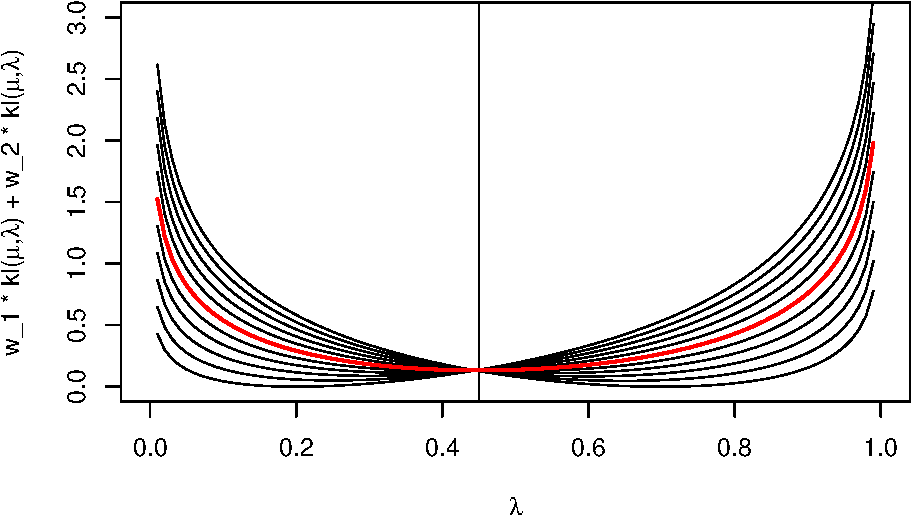
\includegraphics{Draft_files/figure-latex/unnamed-chunk-1-1.pdf}

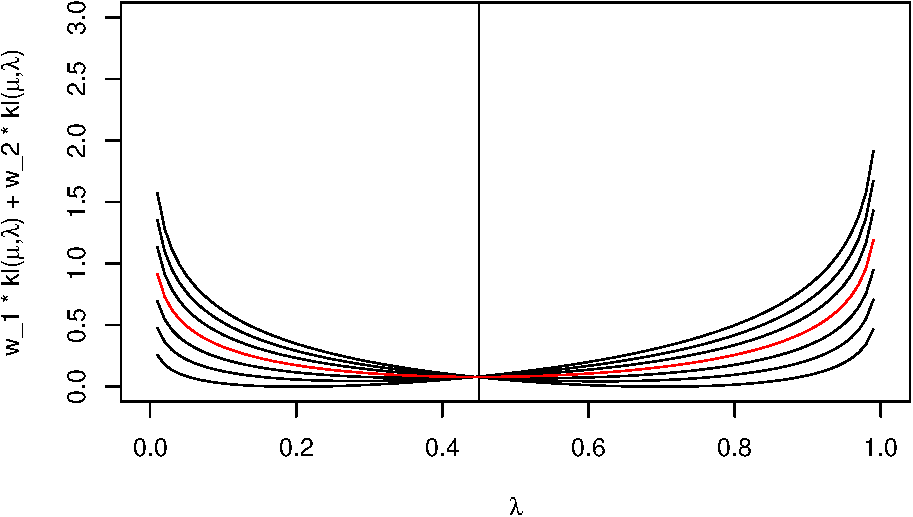
\includegraphics{Draft_files/figure-latex/unnamed-chunk-2-1.pdf}

\subsection{Lower Bound: Theorem and
Proof}\label{lower-bound-theorem-and-proof}

\begin{theorem}[Theorem 1, Locatelli et al., 2016] 
\label{theorem:Locatelli2016Theorem1}
For any sequence of gaps $(d_k)_k$, define a finite set of problems with Gaussian distributions with means corresponding to the gaps, and with variance 1. Lower bound the largest probability of error among these problems for the best possible algorithm as follows. Let $K,T \geq 0$. Let for any $i \leq K$, $d_i \geq 0$. Let $\tau \in \mathbb{R}, \epsilon > 0$.

For $0 \leq i \leq K$, we write $\mathcal{B}^i$ for the problem where the distribution of arm $j \in \{1, \dots, K\}$ is $\mathcal{N}(\tau+d_i+\epsilon, 1)$ if $i \neq j$ and $\mathcal{N}(\tau-d_i-\epsilon, 1)$ otherwise. For all these problems, $H := H_{\tau, \epsilon} = \sum_i (d_i+2\epsilon)^{-2}$ is the same by definition.

It holds that for any bandit algorithm,

\begin{equation*}
\max_{i \in \{0, \dots, K\}} \mathbb{E}_{\mathcal{B}^i} (\mathcal{L}(T)) \geq \exp(-3T/H-4 \log(12(\log(T)+1)K)),
\end{equation*}

where $\mathbb{E}_{\mathcal{B}^i}$ is the expectation according to the samples of problem $\mathcal{B}^i$.
\end{theorem}

\emph{Proof of Theorem \ref{theorem:Locatelli2016Theorem1}}: In Theorem
\ref{theorem:Locatelli2016Theorem1} of Locatelli et al. (2016), a lower
bound for the thresholding bandit problem is shown. The basic idea is as
follows. The problem formulation considered in the paper describes
bandit problems for sub-Gaussian distributions. To show a lower bound,
we show that every algorithm is expected to make a certain error even if
we restrict ourselves to a very restricted scenario. Even then, any
algorithm will have a certain level of risk with which it cannot
distinguish between the actual setting and slightly changed settings
(under which the former answer leads to regret).

To be more specific, consider a case in which we set \(\tau = 0\) and
\(\epsilon = 0\) w.l.o.g. If we then choose all arms to have normally
distributed feedback with means \(\mu_i\), we see that for each arm
\(i\) the distance from the threshold is given by
\(\Delta_i = |\mu_i - \tau| + \epsilon = \mu_i\). Thus, assuming a
variance of 1 for every arm, we have for every arm the distribution
\(\nu_i = \mathcal{N}(\mu_i,1) = \mathcal{N}(\Delta_i,1)\). Furthermore,
define for each arm \(i \in \{1, \dots, K\}\) the alternative
distribution \(\nu_i' = \mathcal{N}(-\Delta_i,1)\). It is easy to see
that in this case, this is equivalent to a ``flip around the
threshold''. Arms that originally have a mean larger than the threshold
have a mean smaller than the threshold after the flip.

The idea now is that every arm \(i \in \{1,\dots,K\}\) generates a
sample for every time point \(t\in \{1, \dots, T\}\) from its
distribution \(\nu_i\) before the algorithm starts to choose arms. Thus,
we have a \(T \times K\) table of realized observations from the product
distribution given by
\(\mathcal{B}^0 = \nu_1^0 \otimes \ldots \otimes \nu_K^0 = \nu_1^0 \otimes \ldots \otimes \nu_K\).
This is a product distribution where the \(K\) different means all lie
above the threshold. We would hope that an algorithm classifies the
means accordingly. However, we will show in what follows that any
algorithm makes a certain error by not being able to distinguish
\(\mathcal{B}^0\) from at least one of \(K\) alternative product
distributions \(\mathcal{B}^i, i \in \{1, \dots, K\}\), of which each
differs only slightly in one arm from the original distribution, and has
the same overall complexity (as defined by
\(H = \sum_{i=1}^K (\Delta_i)^{-2}\)). We require \(K\) different
distributions so that an arm sampling arm \(i\) very often for some
reason will not have a smaller lower bound by chance.

For each of the \(K\) arms, we introduce an alternative model of the
following kind. Before the start of the algorithm, we introduce a slight
variation in the setup. The idea is similar to how one can switch arms
in the pure exploration setup for multi-armed bandits (compare Audibert
et al., 2010; Garivier \& Kaufmann, 2016) to ``confuse'' any algorithm
without introducing additional complexity to the specified problem.
However, since we do not compare arms directly with each other in the
thresholding bandit problem (switching arms would still keep all means
above the threshold), we instead need to flip an arm \(i\) with respect
to the threshold in order to get the alternative model
\(\mathcal{B}_i\). Since the threshold is \(\tau = 0\), we have for the
flipped arm the new distribution \(\nu_i'\) as defined above. Indeed, we
can define the new product distribution
\(B^i = \nu_1^i \otimes \dots \otimes \nu_K^i\) where for
\(k \leq K, \nu_k' := \nu_i \mathbbm{1}_{k \neq i} + \nu_i' \mathbbm{1}_{k=i}\).
This flipping of the arm corresponds to multiplying all random variables
\(X_{i,t}\) of arm \(i\) by \(-1\).

As in Locatelli et al. (2016), we let for \(i \leq K\),
\(\mathbb{P}_{\mathcal{B}^i}\) define the probability distribution
describing all samples that a bandit strategy can potentially collect up
to horizon \(T\), i.e.~according to the samples
\((X_{k,s})_{k\leq K, s \leq T} \sim (\mathcal{B}^i)^{\otimes T}\).
\((T_k)_{k\leq K}\) denotes the number of samples collected on arm \(k\)
until time \(T\).

\subsubsection{Reminder about the goal of the
proof}\label{reminder-about-the-goal-of-the-proof}

At this point, we have defined a finite set of problems of Gaussian
distributions with fixed variance 1 for a given set of set of gaps
between the means of the distributions and the threshold, \((d_k)_k\).
We will now proof a lower bound on the worst case regret of any
algorithm; that is, the maximum error probability that even the best
algorithm makes on this problem.

\subsubsection{Statistical Decision}\label{statistical-decision}

Given our formulation of the regret, the expected regret
\(\mathbb{E}[\mathcal{L}(T)]\) corresponds directly to the probability
of making a wrong classification of any of the \(K\) means. In general,
let \(g\) be a binary decision function, and define
\(\Omega = \{g = 0\}\) and \(\Omega^C = \{g = 1\}\). Assume that the
decision \(T\) distinguishes between two states of the world, \(H_0\)
and \(H_1\). Then our overall error probability is given by
\(P_{H_0}(g=1) + P_{H_1}(g = 0) = P_{H_0}(\Omega^C) + P_{H_1}(\Omega)\).

In our case, \(H_0\) may correspond to the state in which we have
\(\mathcal{B}^0\), and \(H_1\) corresponds to the case where any arm has
been flipped, \(\mathcal{B}^i\). Furthermore, we consider the events in
which the algorithm, making the decision, classifies arm \(i\) as being
above the threshold: \(\mathcal{A}_i = \{i \in \hat{S}_\tau\}\). The
event on which all arms are being classified as above the threshold is
consequently given by \(\mathcal{A} = \bigcap \mathcal{A}_i\). However,
Theorem 1 does not bound the overall regret, but the maximum error
probability on the \(K+1\) different models. We can write this now as

\begin{align}
\max_{i \in \{0, \dots, K\}} \mathbb{E}_{\mathcal{B}^i} (\mathcal{L}(T)) & \geq \max \big( \max_{i \in \{1, \dots, K\}} \mathbb{P}_{\mathcal{B}^i}(\mathcal{A}_i), \mathbb{P}_{\mathcal{B}^0}(\mathcal{A}^C) \big) \\
& = \max \big( \max_{i \in \{1, \dots, K\}} \mathbb{P}_{\mathcal{B}^i}(\mathcal{A}_i), 1 - \mathbb{P}_{\mathcal{B}^0}(\mathcal{A}) \big) \label{LocatelliTheorem1ExpRegret}
\end{align}

In order to give a bound on above equation, we start by considering
\(\mathbb{P}_{\mathcal{B}^i}(\mathcal{A}_i)\). This probability can be
written as the expected change in the likelihood of observed data when
moving from distribution \(P_{\mathcal{B}_0}\) to \(P_{\mathcal{B}_i}\),
times the probability under the original state. In other words, the
probability of event \(\mathcal{A}_i\) under state \(\mathcal{B}^i\) is
given as the probability of \(\mathcal{A}_i\) under the (original) state
\(\mathcal{B}^0\) multiplied by a factor. This factor describes whether
the new distribution increases or decreases the probability of the
event, and is given by the change in the data likelihoods due to moving
from \(\mathcal{B}^0\) to \(\mathcal{B}^i\), expressed as the expected
likelihood ratio under \(\mathcal{B}^0\). By definition, the latter is
equal to the empirical Kullback-Leibler divergence of the two
distributions.

We will define the change of distribution in terms of the empirical
log-likelihood for our case. Then, we will show how to replace the
log-likelihood by the empirical Kullback-Leibler divergence. So let us
first introduce the empirical Kullback-Leibler divergence.

Let every \(\nu_i, \nu_i'\) be dominated by the Lebesgue measure
\(\lambda\). Then their density functions are given by
\(f_i = \frac{\der \nu_i}{\der \lambda}\) and
\(f_i' = \frac{\der \nu_i'}{\der \lambda}\) respectively. For
\(T \geq t \geq 0\), define the empirical Kullback-Leibler divergence as

\begin{align*}
\hat{\KL}_{k,t} & = \frac{1}{t} \sum_{s=1}^{t} \log(\frac{\der \nu_k'}{\der \nu_k}(X_{k,s})) \\
& = \frac{1}{t} \sum_{s=1}^{t} \log \big(\frac{f_k'(X_{k,s})}{f_k(X_{k,s})} \big) \\
& = \frac{1}{t} \log \big( \prod_{s=1}^{t} \frac{f_k'(X_{k,s})}{f_k(X_{k,s})} \big) \\
& \stackrel{\text{iid}}{=} \frac{1}{t} \log \big( \frac{f_k'(X_{k,1}, \dots,X_{k,t})}{f_k(X_{k,1}, \dots,X_{k,t})} \big) \\
& = \frac{1}{t} \log \big( \text{LR}((X_{k,1}, \dots,X_{k,t}), \nu_k', \nu_k) \big)
\end{align*}

Since we consider Gaussian distributions with variance 1, we have
density functions
\(f_i(x) \propto \exp \big(-\frac{1}{2} (x-\Delta_i)^2\big)\) and
\(f_i'(x) \propto \exp \big(-\frac{1}{2} (x+\Delta_i)^2\big)\). Plugging
this into the above definition of the empirical Kullback-Leibler
divergence, we easily see

\begin{align*}
\hat{\KL}_{k,t} & = \frac{1}{t} \sum_{s=1}^{t} \log \big(\frac{\exp \big(-\frac{1}{2} (X_{k,s}+\Delta_k)^2\big)}{\exp \big(-\frac{1}{2} (X_{k,s}-\Delta_k)^2\big)} \big) \\
& = \frac{1}{t} \sum_{s=1}^{t} \log \big( \exp(-\frac{1}{2} (X_{k,s}+\Delta_k)^2 + \frac{1}{2} (X_{k,s}-\Delta_k)^2) \big) \\
& = - \frac{1}{t} \sum_{s=1}^{t} 2 X_{k,s} \Delta_k
\end{align*}

\subsubsection{Change of Distribution}\label{change-of-distribution}

We are now ready to state the change of distribution. As alluded to
above, we consider how the probability changes for the event
\(\mathcal{A}_i\) when we move from \(\mathcal{B}^0\) to
\(\mathcal{B}^i\). When flipping arm \(i\), we only changed the samples
of this arm, that is, the first \(T_i\) observations we got from arm
\(i\) the algorithm took. The change of distribution is then defined as:

\begin{align*}
\mathbb{P}_{\mathcal{B}^i}(\mathcal{A}_i) & = \mathbb{E}_{\mathcal{B}^0} \big[\mathbbm{1}_{\mathcal{A}_i} \text{LR}((X_{i,1}, \dots,X_{i,T_i}), \nu_i', \nu_i) ] \\
& = \mathbb{E}_{\mathcal{B}^0} \big[\mathbbm{1}_{\mathcal{A}_i} \exp (- T_i \hat{\KL}_{i,T_i}) ]
\end{align*}

Obviously, \(\hat{\KL}_{i,T_i}\) depends on the realized samples
\(X_{i,1}, \dots,X_{i,T_i}\). Consequently, we need to find a bound on
\(\hat{\KL}_{i,T_i}\) itself to incorporate the uncertainty involved in
this metric.

\subsubsection{Concentration of the Empirical Kullback-Leibler
Divergence}\label{concentration-of-the-empirical-kullback-leibler-divergence}

For our problem, the Kullback-Leibler divergence of \(\nu_k'\) from
\(\nu_k\) is given by \(\KL_k := KL(\nu_k', \nu_k) = 2\Delta_k^2\).

It is easy to see that

\begin{equation*}
|\hat{\KL}_{k,t} - \KL_{k,t}| = |-\frac{2}{t} \Delta_k \sum_{s=1}^{t}(X_{k,s} - \Delta_k)|
\end{equation*}

itself is a normally distributed random variable with mean zero and a
variance decreasing in \(t\). Thus, one can show as in Locatelli et al.
(2016) that \(\mathbb{P}_{\mathcal{B}^i}(\xi) \geq 3/4\) for the event

\begin{equation}
\xi = \{ \forall k \leq K, \forall t \leq T, |\hat{\KL}_{k,t} - \KL_{k,t}| \leq 4 \Delta_k \sqrt{\frac{\log(4(\log(T)+1)K)}{t}}\}. \label{LocatelliTheorem1EventXi}
\end{equation}

Thus, in order to bound the empirical Kullback-Leibler divergence in our
change of measure, we can consider the intersection of \(\mathcal{A}_i\)
and \(\xi\) as follows and plug in the bound on event \(\xi\):

\begin{align*}
\mathbb{P}_{\mathcal{B}^i}(\mathcal{A}_i) & = \mathbb{E}_{\mathcal{B}^0} \big[\mathbbm{1}_{\mathcal{A}_i} \exp (- T_i \hat{\KL}_{i,T_i}) ] \\
& \geq \mathbb{E}_{\mathcal{B}^0} \big[\mathbbm{1}_{\mathcal{A}_i \cap \xi} \exp (- T_i \hat{\KL}_{i,T_i}) ] \\
& \geq \mathbb{E}_{\mathcal{B}^0} \big[\mathbbm{1}_{\mathcal{A}_i \cap \xi} \exp (- 2 \Delta_i^2 T_i - 4 \Delta_i \sqrt{T_i} \sqrt{\log(4(\log(T)+1)K)}) ]
\end{align*}

Two things are left to do: With \(T_i\), we still have one random
variable left which we cannot leave in our bound. Second, we are
actually not interested in \(\mathbb{P}_{\mathcal{B}^i}(\mathcal{A}_i)\)
but in
\(\max_{i \in \{1,\dots,K\}} \mathbb{P}_{\mathcal{B}^i}(\mathcal{A}_i)\).

\subsubsection{\texorpdfstring{Bounding \(T_i\) for
\(\max_{i \in \{1,\dots,K\}}\mathbb{P}_{\mathcal{B}^i}(\mathcal{A}_i)\)}{Bounding T\_i for \textbackslash{}max\_\{i \textbackslash{}in \textbackslash{}\{1,\textbackslash{}dots,K\textbackslash{}\}\}\textbackslash{}mathbb\{P\}\_\{\textbackslash{}mathcal\{B\}\^{}i\}(\textbackslash{}mathcal\{A\}\_i)}}\label{bounding-t_i-for-max_i-in-1dotskmathbbp_mathcalbimathcala_i}

Part of our bound is
\(\max_{i \in \{1,\dots,K\}} \mathbb{P}_{\mathcal{B}^i}(\mathcal{A}_i)\),
so let's continue with that. In general it holds that
\(\max_{1 \leq i \leq K} (X_1, \dots, X_K) \geq \frac{1}{K}\sum_{i=1}^K X_i\).
Thus we can write:

\begin{align*}
\max_{i \in \{1,\dots,K\}} \mathbb{P}_{\mathcal{B}^i}(\mathcal{A}_i) & \geq \frac{1}{K} \sum_{i=1}^{K} \mathbb{P}_{\mathcal{B}^i}(\mathcal{A}_i) \\
& \geq \frac{1}{K} \sum_{i=1}^{K} \mathbb{P}_{\mathcal{B}^i}(\mathcal{A}_i \cap \xi) \\
& \geq \frac{1}{K} \sum_{i=1}^{K} \mathbb{E}_{\mathcal{B}^0} \big[\mathbbm{1}_{\mathcal{A}_i \cap \xi} \exp (- 2 \Delta_i^2 T_i - 4 \Delta_i \sqrt{T_i} \sqrt{\log(4(\log(T)+1)K)}) ]
\end{align*}

where the second line is again the intersection of \(\mathcal{A}_i\) and
\(\xi\) as before in order to apply the change of distribution in the
third line.

What is left to show before we have our final bound is a bound on
\(T_i\). To show that any algorithm has a certain bound on its error, it
only makes sense that every arm has to pulled at least a certain amount
of times. Consequently, no arm should be pulled exclusively.

First, let \(a = \Delta_i \sqrt{T_i}\) and
\(b = 4\sqrt{\log((4\log(T)+1)K)}\). Then use \(ab \leq a^2 + b^2\) to
write \(ab \leq \Delta_i^2 T_i + 16\log((4\log(T)+1)K)\). And so:

\begin{align*}
\max_{i \in \{1,\dots,K\}} \mathbb{P}_{\mathcal{B}^i}(\mathcal{A}_i) & \geq \frac{1}{K} \sum_{i=1}{K} \mathbb{E}_{\mathcal{B}^0} \big[\mathbbm{1}_{\mathcal{A}_i \cap \xi} \exp (- 3 \Delta_i^2 T_i - 16 \log(4(\log(T)+1)K)) ]
\end{align*}

Furthermore, we know that the sum of the individual arm pulls has to be
equal to the overall number of pulls (equal to the budget in the fixed
budget sense), \(\sum_i T_i = T\), and furthermore we know that
\(T_i>0\). The latter holds since any reasonable algorithm has to check
each arm at least once in our setup. This is because we need to check
each arm's performance in comparison to the threshold. Thus it is easy
to show that
\(\exists i: T_i \leq \frac{T}{H \Delta_i^2} = \frac{T}{(\sum_{i=1}^{K} \Delta_i^{-2}) \Delta_i^2}\).
To see this, assume the opposite:
\(\forall i: T_i > T \frac{\sum_{i=1}^K \Delta_i^2}{\Delta_i^2}\). This
implies however
\(\sum_{i=1}^K T_i > \sum_{i=1}^K T \frac{\sum_{i=1}^K \Delta_i^2}{\Delta_i^2} = T \cdot 1 = T\)
which is a contradiction.

So we can write \((\Delta_i \sqrt{T_i})^2 \leq \frac{T}{H}\). We use
\(\mathcal{A} = \cap_{i=1}^K \mathcal{A}_i\) to write:

\begin{align*}
\max_{i \in \{1,\dots,K\}} \mathbb{P}_{\mathcal{B}^i}(\mathcal{A}_i) & \geq \frac{1}{K} \sum_{i=1}^{K} \mathbb{E}_{\mathcal{B}^0} \big[\mathbbm{1}_{\mathcal{A}_i \cap \xi} \exp (- 3 \Delta_i^2 T_i - 16 \log(4(\log(T)+1)K)) \big] \\
& = \mathbb{E}_{\mathcal{B}^0} \big[\mathbbm{1}_{\mathcal{A} \cap \xi} \frac{1}{K} \sum_{i=1}{K} \exp (- 3 \Delta_i^2 T_i - 16 \log(4(\log(T)+1)K)) \big]
\end{align*}

We write
\(\frac{1}{K} \sum_{i=1}^K \exp(-3T_i \Delta_i^2) \geq \frac{1}{K} \sum_{i=1}^K \exp(-3 T/H) = \exp(-3 T/H)\).
Thus:

\begin{align*}
\max_{i \in \{1,\dots,K\}} \mathbb{P}_{\mathcal{B}^i}(\mathcal{A}_i) & = \mathbb{E}_{\mathcal{B}^0} \big[\mathbbm{1}_{\mathcal{A} \cap \xi} \frac{1}{K} \sum_{i=1}^{K} \exp (- 3 \Delta_i^2 T_i) \exp(-16 \log(4(\log(T)+1)K)) ] \\
& \geq \mathbb{E}_{\mathcal{B}^0} \big[\mathbbm{1}_{\mathcal{A} \cap \xi} \frac{1}{K} \sum_{i=1}^{K} \exp (- 3 \frac{T}{H}) \exp(-16 \log(4(\log(T)+1)K)) ] \\
& = \mathbb{E}_{\mathcal{B}^0} \big[\mathbbm{1}_{\mathcal{A} \cap \xi} \exp (- 3 \frac{T}{H}) \exp(-16 \log(4(\log(T)+1)K)) ] \\
& = \mathbb{P}_{\mathcal{B}^0} (\mathcal{A} \cap \xi) \exp (- 3 \frac{T}{H} -16 \log(4(\log(T)+1)K))
\end{align*}

\subsubsection{Bringing everything
together}\label{bringing-everything-together}

Consider again the risk which we need to bound from equation
\eqref{LocatelliTheorem1ExpRegret}. We bound the maximum expected loss
over all \(\mathcal{B}_i\). By again using the fact that in general
\(\max_{1 \leq i \leq K} (X_1, \dots, X_K) \geq \frac{1}{K} \sum_{i = 1}^K X_i\),
we plug in our previous calculations:

\begin{align}
\max_{i \in \{0, \dots, K\}} \mathbb{E}_{\mathcal{B}^i} (\mathcal{L}(T)) & \geq \max \big( \max_{i \in \{1, \dots, K\}} \mathbb{P}_{\mathcal{B}^i}(\mathcal{A}_i), 1 - \mathbb{P}_{\mathcal{B}^0}(\mathcal{A}) \big) \\
& \geq \frac{1}{2}\mathbb{P}_{\mathcal{B}^0} (\mathcal{A} \cap \xi) \exp (- 3 \frac{T}{H} -16 \log(4(\log(T)+1)K)) + \frac{1}{2}(1 - \mathbb{P}_{\mathcal{B}^0}(\mathcal{A})) \label{LocatelliTheorem1DefinitionOfRisk}
\end{align}

From \eqref{LocatelliTheorem1EventXi} we know that for any
\(i \in \{0, \dots, K\}\), \(\mathbb{P}_{\mathcal{B}^i}(\xi) \geq 3/4\).
Following the argument in Locatelli et al. (2016), we now consider two
cases: \(\mathbb{P}_{\mathcal{B}^0}(\mathcal{A}) \geq 1/2\) and
\(\mathbb{P}_{\mathcal{B}^0}(\mathcal{A}) \leq 1/2\). In the former
case, we can plug in the two probabilities into
\eqref{LocatelliTheorem1DefinitionOfRisk}. If
\(\mathbb{P}_{\mathcal{B}^0}(\mathcal{A}) \geq 1/2\) and
\(\mathbb{P}_{\mathcal{B}^0}(\xi) \geq 3/4\), then
\(\mathbb{P}_{\mathcal{B}^0}(\mathcal{A} \cap \xi) \geq 1/4\). Thus:

\begin{align*}
\max_{i \in \{0, \dots, K\}} \mathbb{E}_{\mathcal{B}^i} (\mathcal{L}(T)) & \geq \max \big( \max_{i \in \{1, \dots, K\}} \mathbb{P}_{\mathcal{B}^i}(\mathcal{A}_i), 1 - \mathbb{P}_{\mathcal{B}^0}(\mathcal{A}) \big) \\
& \geq \frac{1}{2}\mathbb{P}_{\mathcal{B}^0} (\mathcal{A} \cap \xi) \exp (- 3 \frac{T}{H} -16 \log(4(\log(T)+1)K)) + \frac{1}{2}(1 - \mathbb{P}_{\mathcal{B}^0}(\mathcal{A})) \\
& \geq \frac{1}{8} \exp (- 3 \frac{T}{H} -16 \log(4(\log(T)+1)K))
\end{align*}

where we drop the second summand of the second line so that the
inequality holds.

On the other hand, when
\(\mathbb{P}_{\mathcal{B}^0}(\mathcal{A}) \leq 1/2\), then we know that
\(\mathbb{P}_{\mathcal{B}^0}(\mathcal{A} \cap \xi) \leq 1/2\) for any
\(\mathbb{P}_{\mathcal{B}^0}(\xi)\). At the same time
\(1-\mathbb{P}_{\mathcal{B}^0}(\mathcal{A}) = \mathbb{P}_{\mathcal{B}^0}(\mathcal{A^C}) \geq 1/2\).
Consequently,
\(1/4 \leq \frac{1}{2}(1 - \mathbb{P}_{\mathcal{B}^0}(\mathcal{A})) \leq 1/2\),
while
\(\frac{1}{2}\mathbb{P}_{\mathcal{B}^0} (\mathcal{A} \cap \xi) \exp (- 3 \frac{T}{H} -16 \log(4(\log(T)+1)K)) \geq 0\).
And so the stronger lower bound in that case is, as noticed by Locatelli
et al. (2016), given simply by

\begin{align*}
\max_{i \in \{0, \dots, K\}} \mathbb{E}_{\mathcal{B}^i} (\mathcal{L}(T)) & \geq \max \big( \max_{i \in \{1, \dots, K\}} \mathbb{P}_{\mathcal{B}^i}(\mathcal{A}_i), 1 - \mathbb{P}_{\mathcal{B}^0}(\mathcal{A}) \big) \\
& \geq 1 - \mathbb{P}_{\mathcal{B}^0}(\mathcal{A}) = \mathbb{P}_{\mathcal{B}^0}(\mathcal{A^C}) \\
& \geq \frac{1}{2}
\end{align*}

\subsection{Upper Bound: Theorem and
Proof}\label{upper-bound-theorem-and-proof}

\begin{theorem}[Locatelli et al., 2016] \label{theorem:LocatelliTheorem4}
Let $K \geq 0$, $T \geq 2K$, and consider a problem $\mathbb{B}$. Assume that
all arms $\nu_k$ of the problem are R-sub-Gaussian with means $\mu_k$. Let $\tau
\in \mathbb{R}, \epsilon \geq 0$.

Algorithm APT's expected loss is upper bounded on this problem as 
\begin{equation*} \mathbb{E}(\mathcal{L}(T)) \leq \exp
(-\frac{1}{64R^2}\frac{T}{H} + 2 \log (T) + 1)K)) \end{equation*}

where we remind that $H = \sum_i (|\mu_i - \tau | + \epsilon)^{-2}$ and where
$\mathbb{E}$ is the expectation according to the samples of the problem.
\end{theorem}

\emph{Proof of Theorem \ref{theorem:LocatelliTheorem4}:} To prove above
theorem, we first define a favorable event \(\xi\) on which we hope to
make a loss with only a small probability. Indeed, it is the event for
which we want to upper bound the expected loss. As we want to find an
upper bound for the expected loss of the APT algorithm, the event
corresponds to the decision made by it. Given that the APT algorithm's
sampling rule and final decision is based on the empirical mean of each
arm, it will have low expected regret, if it finds empirical mean
estimates \(\hat{\mu}_i(t) = \frac{1}{s} \sum_{t=1}^s X_{i,t}\) that are
close to the true means \(\mu_i\) of the arms. Then, we would expect
arms with \(\hat{\mu}_i(T) > \tau + \epsilon\) to be classified
correctly, and arms with \(\hat{\mu}_i(T) < \tau - \epsilon\) to be
rejected.

Indeed, we have
\(\mathbb{E}(\mathcal{L}(T)) = P(S_{\tau + \epsilon} \cap \hat{S}_\tau^C \neq \emptyset \lor S_{\tau-\epsilon}^C \cap \hat{S}_{\tau} \neq \emptyset)\).
But this just corresponds to
\(P(\{\exists i: ((\mu_i < \tau-\epsilon) \land(\hat{\mu}_i \geq \tau)) \lor ((\mu_i > \tau + \epsilon) \land (\hat{\mu}_i < \tau)))\).
Each of the two \((...)\lor(...)\) conditions corresponds to
\(| \hat{\mu}_i - \mu_i | \geq \epsilon\). It follows that the expected
loss can be rewritten as:
\(\mathbb{E}(\mathcal{L}(T)) = P(\exists i, \exists s: |\hat{\mu}_{i,s} - \mu_i | \geq \epsilon) = P(\xi^C)\).
This is exactly the probability of classifying at least one arm
incorrectly which results in a loss of size 1.

Thus we define as the favorable event as:

\begin{equation} 
\xi = \{\forall i, \forall s: | \hat{\mu}_{i,s} - \mu_i | \leq
\epsilon\} 
\end{equation}

Furthermore, if we write
\(\xi_{i,s} = \{ |\hat{\mu}_{i,s}-\mu_i | \leq \epsilon \}\), then the
following holds by a union bound.

\begin{equation} 
P(\xi) = P(\cap_i \cap_s \xi_{i,s}) = 1 - P(\cup_i \cup_s
\xi_{i,s}^C) \geq 1 - \sum_i \sum_s P(| \hat{\mu}_{i,s} - \mu_i| \geq \epsilon)
\label{theorem2_prob_fav_event} 
\end{equation}

Furthermore, for any \(i \in \{1, \dots, K\}\), for any
\(s \in \{1, \dots, T(i)\}\), with \(X_{it}\) being the random sample
from the R-sub-Gaussian distribution \(v_i\) at time \(t\):

\begin{equation} 
P(| \hat{\mu}_{i,s} - \mu_i| \geq \epsilon) = P(| (\frac{1}{s}
\sum_{t=1}^{s} X_{it} - \mu_i) | \geq \epsilon) = P(| \sum_{t=1}^{s} (X_{it} -
\mu_i) | \geq s \epsilon) 
\end{equation}

where the latter can be bounded by a Hoeffding inequality:

\begin{equation} 
P(| \sum_{t=1}^{s} (X_{it} - \mu_i) | \geq s \epsilon) \leq
2\exp (-\frac{\epsilon^2 s}{2 R^2}) \label{theorem2_hoeffding} 
\end{equation}

The Hoeffding inequality as used here is as follows (compare chapter 2.4
in \href{http://www.stat.yale.edu/~pollard/Books/Mini/Basic.pdf}{David
Pollard (2015)}):

\begin{lemma}[Hoeffding's Inequality] \label{lemma:HoeffdingInequality}
Consider $X_1, \dots, X_T$ independent random variables from R-sub-Gaussian distributions $\nu_i$ with mean $\mu_i$. Then, for any $\epsilon > 0$,

\begin{equation*}
\mathbb{P} \Big( | \sum_{i = 1}^T (X_i - \mu_i) | \geq \epsilon \Big) \leq 2\exp \Big(\frac{-\epsilon^2}{2T R^2}\Big).
\end{equation*}
\end{lemma}

Plugging equation \eqref{theorem2_hoeffding} back into equation
\eqref{theorem2_prob_fav_event}, we get:

\begin{equation}
P(\xi) \geq 1 - \sum_i \sum_s P(| \hat{\mu}_{i,s} - \mu_i| \geq \epsilon) \geq 1 - 2 \sum_i \sum_s \exp (-\frac{\epsilon^2 s}{2 R^2})
\end{equation}

Now, in order to match the performance of the lower bound on the
expected loss derived in Theorem \ref{theorem:Locatelli2016Theorem1}, we
will choose \(\epsilon = \sqrt{\frac{T \delta^2}{Hs}}\). Thus:

\begin{equation}
P(\xi) \geq 1 - 2 \sum_i \sum_s \exp (-\frac{\epsilon^2 s}{2 R^2}) = 1 - 2 \sum_i \sum_s \exp (-\frac{T \delta^2}{2 R^2 H}) \geq 1 - TK \exp(-\frac{T\delta^2}{2R^2H})
\end{equation}

Thus, we do not exactly get the bound from Locatelli et al. (2016)
because we used the Hoeffding inequality instead of the martingale
bound; but the the method should be clear.

What is left now is to show that the favorable event still holds under
the proposed \(\epsilon\), that is, we need to show that under
\(P(\xi) \geq 1 - TK \exp(-\frac{T\delta^2}{2R^2H})\) we still reject
arms that are under \(\tau - \epsilon\) and accept those above
\(\tau + \epsilon\).

\subsubsection{Step 2: Lower Bound on Number of Pulls of Difficult
Arm}\label{step-2-lower-bound-on-number-of-pulls-of-difficult-arm}

In order to see that arms are correctly classified with large
probability, we need to show that they are are pulled sufficiently
often, that is, we have a degree of exploration for each arm \(i\) that
allows us to identify its characteristics. To see this, rewrite the
favorable event of a single arm as follows with \(s = T(i)\):

\begin{equation}
\xi_{i,s} = \{ |\hat{\mu}_{i,s}-\mu_i | \leq \epsilon \} = \{ |\hat{\mu}_{i,s} - \mu_i | \leq \sqrt{\frac{T \delta^2}{H T(i)}}\}
\end{equation}

To make sure that this deviation is small enough, we need to show that
at time \(T\), all \(T(i)\) have a sufficient lower bound and thus all
arms \(i\) have been explored sufficiently to classify correctly with
probability larger \(TK \exp(-\frac{T\delta^2}{2R^2H})\).

To start off, notice that due to the initialization of the APT
algorithm, every \(T_i(T) \geq 1\). Furthermore, we have assumed that
\(T>2K\). Now, at time \(T\), consider an arm \(k\) that has been pulled
\(T_k(T) -1 \geq \frac{(T-K)}{H \Delta^2_k}\) times. That is, it has
been pulled at least proportionally to it's contribution to the overall
hardness of the problem \(H\). Recall
\(H = \sum_{i=1}^K(|\mu_i - \tau|+\epsilon)^-2\) and
\(\delta^2_i = (|\mu_i - \tau | + \epsilon)^2\). To see that such arm
\(k\) exists, assume it does not. Then

\begin{equation*}
T_i(T) - 1 < \frac{T-K}{H \Delta_i^2} \forall i
\end{equation*}\begin{equation*}
T- K = \sum_{i=1}^{K} T_i(T) - 1 < \sum_{i=1}^{K} \frac{T-K}{H \Delta_i^2} = \frac{T-K}{H \Delta_i^2} \sum_{i=1}^{K} \frac{1}{\Delta_i^2} = T-K
\end{equation*}

which is a contradiction.

Consequently, using the assumption \(T>2K\) from above, we have

\begin{equation*}
T_k(T) \geq T_k(T) - 1 \geq \frac{T-K}{H \Delta^2_k} = \frac{T}{2H\Delta_k^2}
\end{equation*}

This states a lower bound on the amount of pulls \(T_k(t)\) for an arm
\(k\) that contributes more than average to the overall hardness of the
problem.

\subsubsection{Step 3: Lower Bound on Number of Pulls of Simple
Arm}\label{step-3-lower-bound-on-number-of-pulls-of-simple-arm}

Next, we would like to derive bounds on the number of pulls of the
remaining arms \(i\) at the time \(t\), the last pull of arm \(k\). To
do so, consider that we are on the favorable event \(\xi\). For every
arm \(i\), it holds:

\begin{equation}
|\hat{\mu}_i(t) - \mu_i | \leq \sqrt{\frac{T \delta^2}{HT_i(t)}} \label{step3_favorable_event} 
\end{equation}

As described in Locatelli et al., using the reverse triangle inequality,
we can write

\begin{IEEEeqnarray*}{rCl}
|\hat{\mu}_i(t) - \mu_i | & = & | (\hat{\mu}_i(t) - \tau) - (\mu_i-\tau) |
\\
& \geq & | |\hat{\mu}_i(t) - \tau| - |\mu_i-\tau| |
\\
& = & | (|\hat{\mu}_i(t) - \tau| + \epsilon) - (|\mu_i-\tau| - \epsilon) |
\\
& = & | \hat{\Delta}_i(t) - \Delta_i |
\end{IEEEeqnarray*}

Consequently, we can again employ the hardness of the task to start
deriving bounds on the number of pulls of the arms:

\begin{equation*}
| \hat{\Delta}_i(t) - \Delta_i | \leq |\hat{\mu}_i(t) - \mu_i | \sqrt{\frac{T \delta^2}{HT_i(t)}}
\end{equation*}

From this, we get

\begin{IEEEeqnarray*}{rlCrl}
\Delta_i - \sqrt{\frac{T \delta^2}{HT_i(t)}} & \leq & \hat{\Delta}_i(t) & \leq & \Delta_i + \sqrt{\frac{T \delta^2}{HT_i(t)}}
\end{IEEEeqnarray*}

and in particular for the arm \(k\) discussed above

\begin{IEEEeqnarray}{rlCrl}
\Delta_k - \sqrt{\frac{T \delta^2}{HT_k(t)}} & \leq & \hat{\Delta}_k(t) & \leq & \Delta_k + \sqrt{\frac{T \delta^2}{HT_k(t)}} \label{delta_hat_k_bounds}
\end{IEEEeqnarray}

To bound \(T_i(t)\), it is helpful to compare \(\Delta_i\) and
\(\Delta_k\) at time \(t\). From the definition of the APT algorithm, we
know that since arm \(k\) has been pulled at time \(t\) (``Pull arm
\(I_{t+1} = \arg \min_i \mathcal{B}_i (t+1)\)''):

\begin{IEEEeqnarray*}{rCl}
\mathcal{B}_k(t) & \leq & \mathcal{B}_i(t)
\\
\sqrt{T_k(t)} \hat{\Delta}_k(t) & \leq & \sqrt{T_i(t)} \hat{\Delta}_i(t)
\end{IEEEeqnarray*}

Thus, every arm \(i\) has a lower bound on it's number of pulls given by
the lower bound for arm \(k\) proportional with it's inverse relative
estimated hardness \(\hat{\Delta}_k(t) / \hat{\Delta}_i(t)\). We can
easily derive a lower bound for the left hand side by plugging in
\eqref{delta_hat_k_bounds}:

\begin{IEEEeqnarray}{rCl}
\sqrt{T_k(t)} (\Delta_k - \sqrt{\frac{T \delta^2}{HT_k(t)}}) & \leq & \mathcal{B}_k(t) 
\\
\sqrt{\frac{T}{2H\Delta_k^2}} (\Delta_k - \sqrt{2}\Delta_k \delta) & = & \sqrt{\frac{T}{H}} (\frac{1}{\sqrt{2}} - \delta)
\\
& \leq & \mathcal{B}_k(t)
\end{IEEEeqnarray}

since \(T_k(t) \geq T/(2H\Delta^2_k)\) and
\(\sqrt{T \delta^2 / (HT_k(t))} \geq \sqrt{T \delta^2 / (H\frac{T}{2H \Delta^2_k})} = \sqrt{2}\Delta_k \delta\).

Next, upper bound \(\mathcal{B}_i(t)\). In contrast to \(T_k(t)\), there
is no lower bound for \(T_i(t)\) available yet that we could plug in.
Thus we derive:

\begin{IEEEeqnarray*}{rCl}
\mathcal{B}_i(t) & = & \sqrt{T_i(t)} \hat{\Delta}_i(t) 
\\
& \leq & \sqrt{T_i(t)} (\Delta_i + \sqrt{\frac{T \delta^2}{H T_i(t)}})
\\
& = & \sqrt{T_i(t)} \Delta_i + \delta \sqrt{\frac{T}{H}}
\end{IEEEeqnarray*}

Combining the two bounds, we get a lower bound on the pulls for every
other arm \(i\):

\begin{IEEEeqnarray*}{rCl}
\Delta_i \sqrt{T_i(t)} + \delta \sqrt{\frac{T}{H}} & \geq & (\frac{1}{\sqrt{2}} - \delta) \sqrt{\frac{T}{H}}
\\
\sqrt{T_i(t)} & \geq & (\frac{1}{\sqrt{2}} - 2\delta) \sqrt{\frac{T}{H}} \frac{1}{\Delta_i}
\\ 
& & \text{(choose $2\delta > 1 / \sqrt{2}$ such that RHS is greater 0)}
% \\
% T_i(t) & \geq & (\frac{1}{2} - 2\sqrt{2} \delta + 4\delta^2) \underbrace{\frac{T}{H} \frac{1}{\Delta_i^2}}_\text{$i$'s share of the budget}
% \\
% T_i(t) & \geq & (1 - 4 \sqrt{2} \delta + 8\delta^2) \frac{T}{2H} \frac{1}{\Delta_i^2}
\end{IEEEeqnarray*}

\subsubsection{Conclusion}\label{conclusion}

As stated before, we require the lower bound on \(T_i(t)\) in order to
show that
\(|\hat{\mu}_i(t) - \mu_i | \leq \sqrt{frac{T \delta^2}{H T_i(t)}}\)
holds for all \(i\). So if we now simply plug in the derived lower
bound, we get:

\begin{equation*}
\mu_i - \Delta_i (\frac{\sqrt{2}\delta}{1-2\sqrt{2}\delta}) \leq \hat{\mu}_i(t) \leq \mu_i + \Delta_i (\frac{\sqrt{2}\delta}{1-2\sqrt{2}\delta})
\end{equation*}

and with \(\lambda := (\frac{\sqrt{2}\delta}{1-2\sqrt{2}\delta}) > 0\):

\begin{equation*}
\mu_i - \Delta_i \lambda \leq \hat{\mu}_i(t) \leq \mu_i + \Delta_i \lambda
\end{equation*}

Under this formulation on \(\xi\), do we accept arms with
\(\mu_i \geq \tau + \epsilon\)? For these arms holds that
\(\Delta_i = \mu_i - \tau + \epsilon\). Consequently:

\begin{IEEEeqnarray*}{rCl}
\mu_i - (\mu_i - \tau + \epsilon) \lambda & \leq & \hat{\mu}_i(t) 
\\ 
\hat{\mu}_i(t) & \geq & \tau \lambda + \mu (1-\lambda) - \epsilon \lambda
\end{IEEEeqnarray*}

The arms are accepted if

\begin{IEEEeqnarray*}{rCl}
\hat{\mu}_i(t) - \epsilon & \geq & 0
\end{IEEEeqnarray*}

Or equivalently as long as

\begin{IEEEeqnarray*}{rCl}
\tau \lambda + \mu(1-\lambda) - \epsilon \lambda - \tau & \geq & 0
\\
\lambda & \leq & \frac{1}{2}
\end{IEEEeqnarray*}

\newpage

\section{Kullback-Leibler Complexity of Pure
Exploration}\label{kullback-leibler-complexity-of-pure-exploration}

In the previous chapter, we have discussed the thresholding bandit
problem as presented in Locatelli et al. (2016). Doing so, we came
across the complexity term \(H = \sum_{i=1}^{K} \Delta_i^{-2}\).
Furthermore, we have noted the fact that an algorithm and bounds based
on \emph{only} the gap between the respective mean and the threshold are
useful in the case of sub-Gaussian problems. Furthermore, even for the
case of Bernoulli arms, which are sub-Gaussian since their feedback is
bounded on \([0,1]\), the gap \(\Delta\) becomes less and less
appropriate for situations in which both \(\mu\) of the Bernoulli, and
\(\tau\) are very close to 0 or 1.

Even though the complexity \(H\) enjoys popularity in the literature of
the best \(m\) arm identification problem, \(m \geq 1\), Kaufmann et al.
(2016) show explicitly that \(H\) is mainly useful for problems of
Gaussian distributions. Indeed, they go so far as to define new measures
of complexity that are based on information theoretic measures Using
those they then display \(H\) as an approximation to their measures in
the case of Gaussian distributions. In turn, this makes apparent that
especially Bernoulli distributions with small means have to be treated
differently.

For the current chapter, we will adopt the notation of Kaufmann et al.
(2016) so that it will be easier to compare the arguments.

\subsection{\texorpdfstring{Complexity of Best-Arm and Top-\emph{m}
Identification}{Complexity of Best-Arm and Top-m Identification}}\label{complexity-of-best-arm-and-top-m-identification}

Instead of the thresholding bandit problem, we now consider the problem
of identifying the best \(m\) out of \(K\) arms, that is, the Top-\(m\)
problem. While we previously looked at a fixed budget formulation, we
now mainly focus on a fixed confidence problem. That is, we hold the
confidence \(1-\delta\) fixed at which a strategy returns the correct
\(m\) arms while trying to find them in a way that minimizes the sample
complexity \(\mathbb{E}_{\nu}[\tau]\), that is, the expected number of
overall draws of the arms. \(\tau\) is also called the stopping time of
the algorithm. Algorithms are supposed to find \(\mathcal{S}_m^*\), the
set of the \(m\) arms with the largest means. If we let
\((\mu_1, \dots, \mu_K)\) be the vector of the means of the arms, then
let \((\mu_{[1]}, \dots, \mu_{[K]})\) be the tuple in which the means
are arranged in decreasing order. For the rest of this chapter, we
consider only settings with arms for which \(\mu_{[m]} > \mu_{[m+1]}\);
that is, the set of the top \(m\) arms, \(\mathcal{S}_m^*\), is unique.
After the sampling phase, we require any algorithm to return the set
\(\hat{S}_m \subset \{1,\dots,K\}\) of \(m\) arms that the algorithm
believes to have the largest means. In the case of fixed confidence, we
fix \(\delta\) at the beginning, such that the algorithm only stops
sampling when
\(\mathbb{P}_{\nu}(\hat{S}_m = \mathcal{S}_m^*) \geq 1-\delta\). We try
to find algorithms who fulfill this as quickly as possible; that is,
they minimize the expected stopping time (or number of draws),
\(\mathbb{E}_{\nu}[\tau]\).

To arrive at the new measure of complexity proposed by Kaufmann et al.
(2016), it will actually make sense to first follow their arguments to a
general lower bound on the sample complexity \(\mathbb{E}_{\nu}[\tau]\)
in the case of fixed confidence problems. This bound is given in their
Theorem 4 (for common confidence levels of \(\delta \leq 0.15\)).

\begin{theorem}[Theorem 4, Kaufmann et al., 2016] \label{theorem:KaufmannEtAlTheorem4}
Let $\nu \in \mathcal{M}_m$, where $\mathcal{M}_m$ is the set of uniquely identifiable bandit models described above. Assume that $\mathcal{P}$ satisfies the continuity conditions in Assumption 3. Any $\delta$-PAC algorithm on $\mathcal{M}_m$ satisfies, for $\delta \leq 0.15$:

\begin{equation*}
\mathbb{E}_{\nu}[\tau] \geq \Big[ \sum_{a \in \mathcal{S}^*_m} \frac{1}{KL(\nu_a, \nu_{[m+1]})} + \sum_{a \notin \mathcal{S}^*_m} \frac{1}{KL(\nu_a, \nu_{[m]})} \Big] \der(1-\delta, \delta),
\end{equation*}

where $\der(x,y) := x \log(x/y) + (1-x) \log((1-x)/(1-y))$ is the binary relative entropy, with the convention that $\der(0,0) = \der(1,1) = 0$.
\end{theorem}

To proof this statement, we assume as before that the arms are ordered
by their means decreasing in size. For a given \(\delta\)-PAC algorithm
\(\mathcal{A} = ((A_t), \tau, \hat{S}_m)\), and under the continuity
conditions (compare Kaufmann et al. (2016)), there exists for every arm
\(a \in \{1, \dots, K\}\) an alternative model
\(\nu' = (\nu_1, \dots, \nu_{a-1}, \nu_a', \nu_{a+1}, \dots, \nu_K)\).
In this alternative model, only arm \(a\) is modified in accordance with
the continuity conditions. Modified in such a way that measured by the
Kullback-Leibler divergence, the arm \(\nu_{m+1}\) is now closer to
\(\nu_a\) than \(\nu_a'\) is to \(\nu_a\), if \(\mu_a > \mu_{m+1}\)
(consequently, \(\mu_a' < \mu_{m+1}\)). On the other hand, if
\(\mu_a < \mu_{m}\), then \(\nu_a'\) will be moved away from \(\nu_a\)
just enough so that \(\nu_a\) is closer to \(\nu_m\) than to \(\nu_a'\)
(consequently, \(\mu_a' > \mu_m\)). These changes in distribution make
the original set of optimal arms, \(\{1,\dots,m\}\) no longer optimal
under the alternative model \(\nu'\). Given that the algorithm returns
\(\hat{S}_m\), we know that for the event
\(\mathcal{E} = (\hat{S}_m = \{1, \dots, m\})\) (which is element of the
by the stopping time \(\tau\) induced \(\sigma\)-Algebra
\(\mathcal{F}_{\tau}\)), that
\(\mathbb{P}_{\nu}(\mathcal{E}) \geq 1-\delta\) and
\(\mathbb{P}_{\nu'}(\mathcal{E}) \leq \delta\) (because fixed confidence
\(\delta\)!).

To now give the lower bound on the expected number of samples,
\(\mathbb{E}_{\nu}[\tau]\), we employ the general lemma given by the
authors for such changes in distribution in bandit models.

\begin{lemma}[Kaufmann et al., 2016] \label{theorem:KaufmannEtAlLemma1}
Let $\nu$ and $\nu'$ be two bandit models with $K$ arms such that for all $a$, the distributions $\nu_a$ and $\nu_a'$ are mutually absolutely continuous. For any almost-surely finite stopping time $\sigma$ with respect to $(\mathcal{F}_t)$,

\begin{equation*}
\sum_{a=1}^{K} \mathbb{E}_{\nu} [N_a(\sigma)] \KL(\nu_a, \nu_a') \geq \sup_{\mathcal{E} \in \mathcal{F}_{\sigma}} \der (\mathbb{P}_{\nu}(\mathcal{E}), \mathbb{P}_{\nu'}(\mathcal{E})),
\end{equation*}

where $\der(x,y)$ is the binary relative entropy as defined above.
\end{lemma}

We can apply this lemma directly on the expected number of draws for
each arm, \(\mathbb{E}_{\nu}[N_a]\). For each arm \(a\), we thus have
\(\KL(\nu_a, \nu_a') \mathbb{E}_{\nu}[N_a] \geq \der (1-\delta, \delta)\).
Using the definition of the alternative model above, we get for every
small but fixed \(\alpha > 0\), for every arm \(a \in \{1, \dots, K\}\)
and each arm \(b \in \{m+1, \dots, K\}\):

\begin{equation*}
\mathbb{E}_{\nu}[N_a] \geq \frac{\der(1-\delta, \delta)}{\KL (\nu_a, \nu_{m+1}) + \alpha}
\end{equation*}

and

\begin{equation*}
\mathbb{E}_{\nu}[N_b] \geq \frac{\der(1-\delta, \delta)}{\KL (\nu_b, \nu_{m}) + \alpha}.
\end{equation*}

We can then let \(\alpha \to 0\), sum the bounds on the individual arms
to get the bound on the overall number of draws:

\begin{equation*}
\mathbb{E}_{\nu}[\tau] = \sum_{a=1}^K \mathbb{E}_{\nu}[N_a] \geq \Big( \sum_{a \in \mathcal{S}_m^*} \frac{1}{\KL(\nu_a, \nu_{[m+1]})} + \sum_{a \notin \mathcal{S}_m^*} \frac{1}{\KL(\nu_a, \nu_{[m]})} \Big) \der(1-\delta, \delta)
\end{equation*}

Given that we will be naturally interested in either very high or very
low confidence of our algorithm, that is, \(P_\nu(\mathcal{E})\) is
either close to 0 or 1, it is possible to use the following
approximation to the binary relative entropy:

\begin{equation}\label{bre_approx}
\forall x \in [0,1], \quad \der(x,1-x) = \der(1-x,x) \geq \log \frac{1}{2.4x}
\end{equation}

And so the final lower bound can be written as

\begin{equation*}
\mathbb{E}_{\nu}[\tau] \geq \Big( \sum_{a \in \mathcal{S}_m^*} \frac{1}{\KL(\nu_a, \nu_{[m+1]})} + \sum_{a \notin \mathcal{S}_m^*} \frac{1}{\KL(\nu_a, \nu_{[m]})} \Big) \log \big(\frac{1}{2.4\delta} \big).
\end{equation*}

\includegraphics{Draft_files/figure-latex/unnamed-chunk-3-1.pdf}

Given this general lower bound for the sampling complexity, or expected
number of draws, it makes sense to define the complexity of a Top-\(m\)
bandit problem using the Kullback-Leibler divergence. After all, besides
the number of arms and the experimenter-chosen confidence, it is just
how close arms are with respect to each other in terms of
Kullback-Leibler divergence that influences the sampling complexity. And
in general, a problem requiring more samples is of course considered to
be more complex (at least with respect to the samples, which is what
needs to be optimized).

Thus, following Kaufmann et al. (2016), define the complexity
\(\kappa_C(\nu)\) for the fixed confidence setting as

\begin{equation}
\kappa_C(\nu) = \inf_{A \, \text{PAC}} \lim_{\delta \to 0} \sup \frac{\mathbb{E}_{\nu}[\tau_{\delta}]}{\log \frac{1}{\delta}}.
\end{equation}

So if we were to plug in the lower bound on the sampling complexity, we
would arrive at a complexity measure that basically depends only on the
Kullback-Leibler measuring for each arm how far it is away from the
border between the two groups of arms. To see this, consider the lower
bound on the complexity measure given in Kaufmann et al. (2016):

\begin{equation*}
\kappa_C(\nu) \geq \sum_{a \in \mathcal{S}_m^*} \frac{1}{\KL(\nu_a, \nu_{[m+1]})} + \sum_{a \notin \mathcal{S}_m^*} \frac{1}{\KL(\nu_a, \nu_{[m]})}
\end{equation*}

Given this description, we can already note that an intuitive extension
of this complexity notion to the thresholding bandit problem might
involve replacing \(\mu_{[m]}\) and \(\mu_{[m+1]}\) by the actual
threshold \(\tau\) (notation in Locatelli et al.) that divides the group
above the threshold from the group below the threshold. In that case,
the previously used \(\alpha\) might be very similar to the \(\epsilon\)
used in Locatelli et al. (2016).

To get there, however, at least two important steps remain. First, we
need to define a complexity for the fixed budget problem. Second, we
need to create algorithms that can match the lower bound.

Kaufmann et al. are able to provide a bound on their complexity measure
in the fixed budget case, however only in the case of \textbf{two-armed}
bandit models. As demanded in their paper, a fixed-budget algorithm is
called consistent if the failure probability
\(p_t(\nu) := \mathbb{P}_{\nu}(\hat{S}_m \neq S^*_m)\) tends to zero as
the number of samples goes to infinity. Also, define the complexity in
the fixed-budget setting as follows:

\begin{equation}
\kappa_B(\nu) = \inf_{A \, \text{consistent}} \big(\lim_{t \to \infty} \sup - \frac{1}{t} \log p_t(\nu)\big)^{-1}.
\end{equation}

Given this definition, one can interpret the bound given in Theorem 12
of Kaufmann et al. directly as a lower bound on the complexity
\(\kappa_B(\nu)\) (note the inverse).

\begin{theorem}[Theorem 12, Kaufmann et al., 2016] \label{theorem:KaufmannEtAlTheorem12}
Let $\nu = (\nu_1, \nu_2)$ be a two-armed bandit model such that $\mu_1 > \mu_2$. In the fixed-budget setting, any consistent algorithm satisfies:

\begin{equation*}
\lim_{t \to \infty} \sup - \frac{1}{t} \log p_t(\nu) \leq \inf_{(\nu_1', \nu_2') \in \mathcal{M}: \mu_1' < \mu_2'} \frac{\KL(\nu_1', \nu_1) + \KL(\nu_2', \nu_2)}{2}
\end{equation*}
\end{theorem}

For a proof, consider first the two different bandit models, \(\nu\) and
\(\nu'\), where we fix without loss of generality that \(a^* = 1\) is
the best arm in \(\nu\), while \(a^* = 2\) in \(\nu'\). Note that in
this case we don't necessarily try to fool the algorithm by a change of
distribution. Indeed, we want the algorithm \(\mathcal{A}\) to be
consistent for both problems. Since we are in the fixed-budget setting,
the stopping time is fixed at \(\tau = t\). Even though the correct
decision differs between the two problems, we focus on the event
\(A = (\hat{S}_1 = 1)\). Given the formulation in Kaufmann et al.
(2016), we have \(A \in \mathcal{F}_t = \mathcal{F}_{\tau}\). Now, we
can apply Lemma 1 as before, as it in essense gives a measure of how
different two bandit models are. Here, we want to know how different
\(\nu\) is from \(\nu'\), and so, given we have only two arms,

\begin{equation*}
\mathbb{E}_{\nu'}[N_1(t)]\KL(\nu_1', \nu_1) + \mathbb{E}_{\nu'}[N_2(t)]\KL(\nu_2', \nu_2) \geq \der(\mathbb{P}_{\nu'}(A),\mathbb{P}_{\nu}(A)))
\end{equation*}

The expectations were chosen with respect to \(\nu'\) in order to allow
the for the following: We have \(p_t(\nu) = 1 - \mathbb{P}_{\nu}(A)\)
and \(p_t(\nu') = \mathbb{P}_{\nu'}(A)\) (since \(A\) is wrong in
\(\nu'\)). But since algorithm \(\mathcal{A}\) is consistent for both
\(\nu\) and \(\nu'\), we know that there should exist some number of
samples such that the probability of event \(A\) is bigger in setting
\(\nu\) (where it is the correct decision), than in setting \(\nu'\)
(where this would be a wrong decision and failure). Thus, for every
\(\epsilon > 0\), there exists \(t_0(\epsilon)\) such that for all
\(t \geq t_0(\epsilon)\),
\(\mathbb{\nu'}(A) \leq \epsilon \leq \mathbb{P}_\nu(A)\). Consequently,
if we plug in the bound of \(\epsilon\) for \(\mathbb{P}_{\nu'}(A)\),
then

\begin{align*}
\mathbb{E}_{\nu'}[N_1(t)]\KL(\nu_1', \nu_1) + \mathbb{E}_{\nu'}[N_2(t)]\KL(\nu_2', \nu_2) & \geq \der(\epsilon,1-p_t(\nu))) \\
& = \epsilon \log \frac{\epsilon}{1-p_t(\nu)} + (1-\epsilon) \log \frac{1-\epsilon}{p_t(\nu)} \\
& \geq (1-\epsilon) \log \frac{1-\epsilon}{p_t(\nu)} + \epsilon \log \epsilon.
\end{align*}

Let \(\epsilon\) go to zero so that

\begin{align*}
\mathbb{E}_{\nu'}[N_1(t)]\KL(\nu_1', \nu_1) + \mathbb{E}_{\nu'}[N_2(t)]\KL(\nu_2', \nu_2)
& \geq \log \frac{1}{p_t(\nu)} = -\log p_t(\nu).
\end{align*}

Dividing both sides by \(t\) and taking the limsup, we arrive at

\begin{align*}
\lim_{t \to 0} \sup - \frac{1}{t} \log p_t(\nu)
& \leq \lim_{t \to 0} \sup \frac{1}{t} \sum_{a=1}^2 \mathbb{E}_{\nu'}[N_a(t)] \KL(\nu_a', \nu_a) \\
& \leq \max_{a=1,2} \KL(\nu_a', \nu_a),
\end{align*}

where the last line follows from the fact that the
\(\frac{1}{t} \sum_{a=1}^2 \mathbb{E}_{\nu'}[N_a(t)]\) part creates a
weighted average of the two divergences \(\KL(\nu_a', \nu_a)\). As noted
in Kaufmann et al. (2016), one arrives at the final result by choosing
\(\mu_1'\), \(\mu_2'\) so that
\(| \KL(\nu_1', \nu_1) - \KL(\nu_2', \nu_2) |\) is as small as possible.

Note that while deriving the lower bound on the complexity measure, we
have also derived the following lower bound on the failure probability
for the two-armed fixed-budget bandit:

\begin{equation*}
p_t(\nu) \geq \exp \big(- \sum_{a=1}^2 \mathbb{E}_{\nu'}[N_a(t)] \KL(\nu_a', \nu_a) \big)
\end{equation*}

or, to not rely on the share of samples attributed to each arm,

\begin{equation*}
p_t(\nu) \geq \exp \big(- \max_{a=1,2} \KL(\nu_a', \nu_a) \big).
\end{equation*}

\textbf{Mention something about the fact that we were not able to do
this for more than 2 arms and top-m bandits. How could it be extended to
that? How could it be extended to the threshold bandit?}

As noted by Kaufmann et al. (2016), the advantage of this lower bound is
that it makes the complexity in the fixed-confidence and the
fixed-budget setting directly comparable. The disadvantage of course
being that the result only holds for two-armed models. While the authors
were not able to derive directly comparable lower bounds for the
Top-\(m\) case, they did derive a first lower bound in the Gaussian case
with equal variances. While we would like to move beyond Gaussian
distributions in the work at hand, the idea for the proof might show a
way of how the ideas can be transferred to the thresholding bandit
problem. We first state the result and then discuss the proof.

\begin{lemma}[Lemma 15, Kaufmann et al., 2016] \label{theorem:KaufmannEtAlLemma15}
Let $\nu$ and $\nu'$ be two bandit models such that $S^*_m(\nu) \neq S*_m(\nu')$. Then

\begin{equation*}
\max \big( \mathbb{P}_{\nu}(S \neq S^*_m(\nu)), \mathbb{P}_{\nu'}(S \neq S^*_m(\nu')) \big) \geq \frac{1}{4} \exp \Big(-\sum_{a=1}^{K} \mathbb{E}_{\nu}[N_a] \KL(\nu_a, \nu_a') \Big).
\end{equation*}
\end{lemma}

The following theorem only holds in the case of Gaussian bandit models
with equal known variance.

\begin{theorem}[Theorem 17, Kaufmann et al., 2016] \label{theorem:KaufmannEtAlTheorem17}

Let $\mathcal{M}_m = \{\nu = (\nu_1, \dots, \nu_K): \nu_a = \mathcal{N}(\mu_a, \sigma^2), \mu_a \in \mathbb{R}, \mu_{[m]}\neq \mu_{[m+1]}\}.$ Furthermore, let $\nu$ be such that $\mu_1 > \dots > \mu_m > \mu_{m+1} > \dots > \mu_K$, and let

\begin{equation*}
H +(\nu) = \sum_{a=1}^m \frac{2\sigma^2}{(\mu_a - \mu_{m+1})^2}, \quad H^-(\nu) = \sum_{a=m+1}^K \frac{2\sigma^2}{(\mu_m - \mu_a)^2} \quad
and \quad
H(\nu) = H^+(\nu) + H^-(\nu).
\end{equation*}

There exists $a \in {1, \dots, m}$ and $b \in \{m+1, \dots, K\}$ such that the bandit model $\nu^{[a,b]}$ described in Figure 4 (Kaufmann et al., 2016) satisfies $H(\nu^{[a,b]}) < H(\nu)$ and is such that

\begin{equation*}
\max \big( p_t(\nu),p_t(\nu^{[a,b]})\big) \geq \frac{1}{4} \exp \big(-\frac{4t}{\bar{H}(\nu)}\big), \quad where \quad \bar{H}(\nu) = \frac{H(\nu) \min(H^+(\nu),H^-(\nu))}{H(\nu)+\min(H^+(\nu),H^-(\nu))}
\end{equation*}
\end{theorem}

Given that we are again in the Top-\(m\) setting, the proof idea is
similar to the proof of Theorem \ref{theorem:KaufmannEtAlTheorem4} in
that we again consider problems where we switch arms around the limit
seperating the two groups of arms as given implicitly by \(\mu_{[m]}\)
and \(\mu_{[m+1]}\). The hope here being that these methods could be
applied to the thresholding bandit problem where the threshold of course
gives the limit between the arms above and below the threshold. As we
have seen in chapter 1, this flip around the threshold was of course
used in the proof of the lower bound in Theorem 1 of Locatelli et al.
(2016). However, there, again, the distributions were assumed to be
Gaussian. This brings the big advantage that the Kullback-Leibler
divergence becomes symmetric, and the feedback can take values on all
\(\mathbb{R}\). And by using the complexity measure \(H(\nu)\), it is
also clear that there exists an arm that is undersampled with respect to
its contribution to the overall complexity of the problem (or sampled
exactly according to its contribution), which leads to leads to a
convenient upper bound on this arms number of draws which is again
employed in both the proof of Theorem
\ref{theorem:KaufmannEtAlTheorem17} and in Locatelli et al. (2016). It
is not clear yet, whether the same can also be done with other
complexity measures.

We do not repeat the proof here for now.

See p20!

What remains is to present algorithms that are able to match the lower
bounds derived so far.

\subsubsection{Matching algorithm
strategies}\label{matching-algorithm-strategies}

Given these lower bounds, all that is left is to find algorithms which
are able to match the complexity. Sadly, not straightforward for
Bernoullis.

Kaufmann et al. (2016) do not present algorithms matching the lower
bound of Theorem \ref{theorem:KaufmannEtAlTheorem17}. They do consider
algorithms that connect to Theorem \ref{theorem:KaufmannEtAlTheorem4}
and Theorem \ref{theorem:KaufmannEtAlTheorem12}.

Given that Locatelli et al. (2016), and thus the problem we mostly
consider in this thesis, is in the fixed-budget setting, we are most
interested in the matching strategies for Theorem
\ref{theorem:KaufmannEtAlTheorem12}. However, given that the lower bound
applies only to two-armed bandits, the algorithms are of limited
practical interest. Furthermore, the algorithms proposed require
knowledge that is in general not available upfront.

For the example of Gaussian distributions, the knowledge of the
(potentially different) variance is assumed which enables a strategy
that pulls each arm proportional to its variance.

Even worse is the case of Bernoulli two-armed bandit models where the
proposed algorithm requires knowledge about the true parameters of the
distributions. That this limits the practical interest is also noted by
the authors of Kaufmann et al. (2016). Thus, they suggest to use uniform
sampling strategies in the case of two-armed Bernoulli bandits, and show
that there is not much to be lost by doing so.

Thus, Kaufmann et al. (2016) join a number of other papers like Audibert
et al. (2010) and Kaufmann and Kalyanakrishnan (2013) which struggle to
find matching strategies in the fixed-budget setting that do not rely on
knowledge of parameters or the complexity of the problem.

In contrast, Kaufmann et al. (2016) are able to show that their
complexity measure derived for the fixed-confidence setting,
\(\kappa_C(\nu)\), can be upper-bounded using the upper bound of the
sample complexity (number of pulls) given for the KL-LUCB algorithm in
Kaufmann and Kalyanakrishnan (2013). Consequently, in the case of
exponential family bandits, the complexity \(\kappa_C(\nu)\) is bounded
as given in equation (6) in Kaufmann et al. (2016):

\begin{equation*}
\sum_{a \in S^*_m} \frac{1}{K(\theta_a, \theta_{[m+1]})} + \sum_{a \notin S^*_m} \frac{1}{K(\theta_a,\theta_{[m]})} \leq \kappa_C(\nu) \leq 24 \min_{\theta \in [\theta_{[m+1]},\theta_{[m]}]} \sum_{a=1}^{K} \frac{1}{K^*(\theta_a, \theta)},
\end{equation*}

where \(K(\theta, \theta') = \KL(\nu_{\theta}, \nu_{\theta'})\) for
\((\theta, \theta') \in \Theta^2\) was defined as the shorthand for the
Kullback-Leibler divergence for two distributions from the exponential
family parameterized by \(\theta\) and \(\theta'\) respectively.
\(K^*(\theta,\theta') = K(\theta^*, \theta)\) is the Chernoff
distribution between the two distributions, where \(\theta^*\) is chosen
so that \(K(\theta^*,\theta) = K(\theta^*, \theta')\).

\subsection{Optimal Best Arm
Identification}\label{optimal-best-arm-identification}

A very similar application of the KL divergence has been given in
Garivier and Kaufmann (2016) to derive a lower bound on the sample
complexity in the case of best arm identification. In particular, the
transportation Lemma 1 is used again. And a matching algorithm for
\(K \geq 2\) arms is proposed.

Talk about: - Not a simple sum of squares - Idea of algorithm: Equalize
the probability of all wrong decisions

In Garivier and Kaufmann (2016), the authors are able to derive a
somewhat similar lower bound on the sample complexity of a \(K\)-armed
bandit in the single best arm identification problem with fixed
confidence. Additionally, they provide a \(\delta\)-PAC algorithm
achieving said bound asymptotically.

In particular, the authors pick up Lemma 1 from Kaufmann et al. (2016)
-- which we discussed above -- to derive the lower bound. While
presenting these results, we try to stick as much as possible with the
notation used so far. In particular, we let for distributions
\(\nu_{\theta}\) from a canonical exponential family, which can be
parameterized by its mean \(\stackrel{.}{b}(\theta) = \mu\) and thus be
written as \(\nu^{\mu}\); for these, we continue to write the
Kullback-Leibler divergence as

\begin{equation*}
\KL(\mu, \mu') = \KL(\nu^{\mu},\nu^{\mu'}) = \KL(\nu_{\theta},\nu_{\theta'}) = \KL(\nu, \nu')
\end{equation*}

while \(d(x,y)\) continues to represent the binary relative entropy.

As we will consider only problems with exponential family distributions,
the distributions can be parameterized by their means. Therefore, if we
let \(\mathcal{S}\) to be a set of bandit models with \(K\)
distributions each, then each model is fully defined by a vector
\(\bm{\mu} = (\mu_1, \dots, \mu_K)\). Assume that every
\(\bm{\mu} \in \mathcal{S}\) has a unique maximum given by
\(a^*(\bm{\mu})\) such that
\(\mu_{a^*} > \max_{a \neq a^*(\bm{\mu})} \mu_a\). In order to fix the
confidence, we specify the risk \(\delta\). The strategies corresponding
to this risk are called \(\delta\)-PAC if for every
\(\bm{\mu} \in \mathcal{S}\),
\(\mathbb{P}_{\bm{\mu}}(\tau_{\delta} < \infty) = 1\) (the strategy ends
surely after a finite number of samples) and
\(\mathbb{P}_{\bm{\mu}}(\hat{a}_{\tau_{\delta}} \neq a^*) \leq \delta\)
(the probability of picking not the optimal arm is smaller than the
fixed risk). As in Garivier and Kaufmann (2016), we introduce the set of
problems for which the optimal arm is different from the one in
\(\bm{\mu}\):

\begin{equation*}
\text{Alt}(\bm{\mu}) := \{\bm{\lambda} \in \mathcal{S}: a^*(\bm{\lambda}) \neq a^*(\bm{\mu})\}
\end{equation*}

where \(\bm{\lambda}\) is the vector of means defining the distributions
of the alternative problem to \(\bm{\mu}\). Lastly, we have the set of
probability distributions on the arms \(\mathcal{A}\):
\(\Sigma_K = \{w \in \mathbb{R}_{+}^K: w_1 + \dots + w_K = 1\}\).
\marginpar{Give more intuition for what these probability distributions are}
We are now ready to state the theorem.

\begin{theorem}[Theorem 1, Garivier and Kaufmann, 2016] \label{theorem:GarivierKaufmannTheorem1}
Let $\delta \in (0,1)$. For any $\delta$-PAC strategy and any bandit model $\bm{\mu} \in \mathcal{S}$,

\begin{equation*}
\mathbb{E}_{\bm{\mu}} [\tau_{\delta}] \geq T^*(\bm{\mu}) \text{\em{d}}(\delta,1-\delta),
\end{equation*}

where 

\begin{equation} \label{eq:GarivierKaufmann_Theorem1_Game}
T^*(\bm{\mu})^{-1} := \sup_{w \in \Sigma_K} \inf_{\bm{\lambda} \in \text{\em{Alt}}(\bm{\mu})} \left( \sum_{a=1}^K w_a \text{\em{KL}}(\mu_a, \lambda_a)\right).
\end{equation}
\end{theorem}

And so we see that the two bounds on the sample complexity (one for
Top-\(m\), one for best arm identification) differ only in the way that
they build the sum of Kullback-Leibler divergences over the \(K\) arms.
In contrast to Theorem \ref{theorem:KaufmannEtAlTheorem4}, here the
contribution of each arm through its KL-divergence is weighted. The
difference is that while we were able to very clearly describe the
change of distribution in the Top-\(m\) case for each arm -- for each
arm, we specified an alternative model that yields a new set of \(m\)
optimal arms -- we now consider all alternative models that yield a
different best arm than the model \(\bm{\mu}\). In the previous theorem,
we sum over the complexity of each individual arm, as the change in
distribution only ever touches one arm, thus leading to a KL-divergence
of 0 for the other arms while still changing the optimal set. Here, we
consider all instances of alternative models \(\bm{\lambda}\), and thus
also those in which several arms are modified (and thus have a
KL-divergence unequal 0 in the result of Lemma 1).

\emph{Proof of Theorem \ref{theorem:GarivierKaufmannTheorem1}}: As
stated before, we let \(\delta \in (0,1)\),
\(\bm{\mu} \in \mathcal{S}\), and only consider \(\delta\)-PAC
strategies. As before, \(N_a(t)\) describes the random number of pulls
of arm \(a\) until time \(t\), for all \(t\geq 1\). Again, Lemma
\ref{theorem:KaufmannEtAlLemma1} states how the failure probability
\(\delta\) relates to the expected number of draws of each arm given two
models which differ in their optimal arm, and where it is evaluated
based on the Kullback-Leibler divergence for each pair of arms how much
the two models differ:

\begin{equation*}
\forall \lambda \in \mathcal{S}: a^*(\lambda) \neq a^*(\mu), \sum_{a=1}^K \KL(\mu_a,\lambda_a)\mathbb{E}_{\bm{\mu}}[N_a(\tau_{\delta})] \geq \d(\delta, 1- \delta).
\end{equation*}

As mentioned, we now do not consider a specific alternative for each
arm, but instead look at the infimum over all the possible alternatives,
and use the fact that
\(\mathbb{E}_{\bm{\mu}}[\tau_{\delta}] = \sum_{a=1}^K \mathbb{E}_{\bm{\mu}}[N_a(\tau_{\delta})]\):

\begin{align*}
\der(\delta, 1-\delta) & \leq \inf_{\lambda \in \text{Alt}(\bm{\mu})} \mathbb{E}_{\bm{\mu}}[\tau_{\delta}] \Big(\sum_{a=1}^K \frac{\mathbb{E}_{\bm{\mu}}[N_a]}{\mathbb{E}_{\mu}[\tau_{\delta}]} \KL(\mu_a, \lambda_a)\Big) \\
& = \mathbb{E}_{\bm{\mu}}[\tau_{\delta}] \inf_{\lambda \in \text{Alt}(\bm{\mu})} \Big(\sum_{a=1}^K \frac{\mathbb{E}_{\bm{\mu}}[N_a]}{\mathbb{E}_{\mu}[\tau_{\delta}]} \KL(\mu_a, \lambda_a)\Big) \\
& \leq \mathbb{E}_{\bm{\mu}}[\tau_{\delta}] \sup_{w \in \Sigma_K} \inf_{\lambda \in \text{Alt}(\bm{\mu})} \Big(\sum_{a=1}^K w_a \KL(\mu_a, \lambda_a)\Big).
\end{align*}

As stated in Garivier and Kaufmann (2016), the term
\(\frac{\mathbb{E}_{\bm{\mu}}[N_a]}{\mathbb{E}_{\mu}[\tau_{\delta}]}\)
gives the fraction of draws each arm receives. This value, however,
depends on the used algorithm. To make it hold for any \(\delta\)-PAC
algorithm, it is replaced by the supremum over \(\Sigma_K\), which is
the distribution over these fractions for any \(\mathcal{A}\), that is,
for any \(\delta\)-PAC strategy.

This lower bound can be interpreted as a Minimax game, where the
experimenter has to choose the share of samples he attributes to each
arm in a way that is optimal given that nature will respond and choose
the most difficult alternative model given his weights. Thus, to make
the lower bound practical, it is a matter of finding the optimal weights
\(w^*(\bm{\mu})\). This step did not occur in the previous lower bound,
as the alternative models were made specific by changing the
distribution of one arm with respect to the ``border'' between the two
groups of arms.

In any case, the existence of the optimal weights suggests an algorithm
that keeps track of the share of samples that is attributed to each arm
and makes sure that it stays close to the optimum until some decision
rule assures that the \(\delta\)-PAC condition is fulfilled.

Indeed, the optimal weights will lead to a sampling structure in which
arms are drawn in such a way ensuring that their individual failure
probabilities are at the same level. Take a situation where the
currently best arm \(\hat{\mu}_1\) is the best arm. Then, we calculate
for each arm the risk that actually it is better than arm 1. Since the
arms are assumed to be independent, the we only have to compare every
arm individually to arm 1. Given that, it makes sense that we don't want
to disregard an arm that has a high probability of being better than arm
1. Assuming arm 1 is actually the best arm, we would an algorithm that
ensures a low failure probability on all arms, thus equalizing the
failure probability for every arm compared to arm 1.

This is exactly what happens when we look for the proportions
\(w \in \Sigma_K\) that minimize the cost from a change in
distributions, that is, the term
\(F(\bm{\mu}, \bm{w}) = \inf_{\bm{\lambda} \in \text{Alt}(\bm{\mu})} \Big(\sum_{a= 1}^K w_a \KL(\mu_a, \lambda_a)\Big)\).
In the proof of Lemma 3 of Garivier and Kaufmann, it is shown that
nature, selecting the alternative model \(bm{\lambda}\) will always pick
an alternative model in which only a single arm \(a\) is changed such
that \(\lambda_a > \lambda_1\) since

\begin{align*}
T^*(\bm{\mu})^{-1} & = \sup_{w \in \Sigma_K} \min_{a \neq 1} \inf_{\bm{\lambda} \in \mathcal{S}: \lambda_a > \lambda_1} \sum_{a=1}^K w_a \KL(\mu_a, \lambda_a)  \\
& = \sup_{w \in \Sigma_K} \min_{a \neq 1} \inf_{\bm{\lambda}: \lambda_a \geq \lambda_1} [w_1 \KL(\mu_1, \lambda_1)+w_a \KL(\mu_a, \lambda_a)].
\end{align*}

Consequently, \(w\) will be chosen so as to minimize \(T^*(\bm{\mu})\)
no matter which arm \(a\) was picked. It is a minimax game, so the ideal
solution is to keep for each arm \(a \neq 1\) the term
\(w_1 \KL(\mu_1, \lambda_1) + w_a \KL(\mu_a, \lambda_a)\) at the same
level. Garivier and Kaufmann show that this can be written in terms of
the Jenson-Shannon divergence, defined for every \(\alpha \in [0,1]\) as

\begin{equation*}
I_{\alpha}(\mu_1, \mu_2) := \alpha \KL(\mu_1, \alpha \mu_1 + (1-\alpha) \mu_2) + (1-\alpha) \KL(\mu_2, \alpha \mu_1 + (1-\alpha) \mu_2).
\end{equation*}

Using this notation, the optimal proportions can be written as

\begin{equation*}
w^*(\bm{\mu}) = \arg \max_{w \in \Sigma_K} \min_{a \neq 1} (w_1 + w_a) I_{\frac{w_1}{w_1+w_a}}(\mu_1, \mu_a)
\end{equation*}

which let's us furthermore conclude that these quantities are equal for
all \(a,b \in \{2,\dots, K\}\) with

\begin{equation*}
(w_1^* + w_a^*) I_{\frac{w_1^*}{w_1^*+w_a^*}}(\mu_1, \mu_a) = (w_1^* + w_b^*) I_{\frac{w_1^*}{w_1^*+w_b^*}}(\mu_1, \mu_b),
\end{equation*}

which is simply the statement in Lemma 4 of Garivier and Kaufmann
(2016).

And so by assuring the reader that there are ways to compute \(w_a^*\)
and \(T^*\) given \(\bm{\mu}\) (see chapter 2.2 in Garivier and Kaufmann
(2016)), we can now introduce the \emph{Track-and-Stop} strategy given
in Garivier and Kaufmann (2016) that is able to match the lower bound by
the intuition given above.

When going from theory to algorithm, the obvious problem is of course
that we do no longer know \(\bm{\mu}\) and thus cannot simply calculate
the optimal weights. Instead, we are estimating the maximum likelihood
estimates \(\hat{\mu}(t) = (\hat{\mu}_1(t), \dots, \hat{\mu}_K(t))\) of
the true mean at the current round \(t\) and need to base our weights
based on these. It is however problematic to rely on these sample means
as we are inherently unsure about them. And so wrong estimates, which
naturally occur most easily in the beginning when not many samples have
been pulled, are prone to lead to wrong weights. Thus, if a wrong
estimate \(\hat{\mu}_a\) for arm \(a\) leads to a small weight \(w_a\),
then neither the estimate nor the weight will be correct soon. Thus,
Kaufmann and Garivier conclude that ``a naive plug-in sampling rule
sometimes fails''. They propose to enforce a certain minimum level of
exploration to make sure that arms that erroneously received a very
small weight will be further explored regardless.

A very intuitive fix to this problem is the solution proposed in Lemma 8
of Garivier and Kaufmann (2016), with their \(D-Tracking\) rule.
Basically, whenever an arm has received a very low number of pulls
\(N_a(t)\) given the number of iterations so far, \(t\) and the number
of arms \(K\) that have to share the samples, pull the arm that has
received the smallest amount of samples so far. Else, pull the arm which
number of pulls so far \(N_a(t)\) is the furthest away from what its
optimal share \(t\cdot w^*_a(\hat{\bm{\mu}}(t))\) would be. Given this
sampling rule, the authors can show in their Proposition 9 that the
empirical proportion of draws converges in probability to the optimal
weights given the true means.

When combining this sampling rule with an appropriate stopping rule, the
authors are able to prove in Theorem 14 an upper bound on the expected
sampling complexity \(\mathbb{E}_{\mu}[\tau_{\delta}]\). The stopping
rule ensures that the algorithm explores sufficiently to promise a risk
smaller than \(\delta\), while stopping as soon as possible. Given that
the sampling rule is independent of this stopping rule, the rule boils
down to a statistical test at every iteration and thus is a sequential
test based on the current estimate of \(\hat{\bm{\mu}}\). The Chernoff's
Stopping Rule proposed in Garivier and Kaufmann (2016) calculates for
each arm \(a\in \mathcal{A}\) the Generalized Likelihood Ratio statistic
with every arm \(b \in \mathcal{A}^{\setminus a}\), which for
\(\hat{\mu}_a(t) \geq \hat{\mu}_b(t)\) can be written as

\begin{equation*}
Z_{a,b}(t) = - Z_{b,a} = N_a(t) \KL(\hat{\mu}_a(t),\hat{\mu}_{a,b}(t)) + N_b(t) \KL(\hat{\mu}_{b}(t), \hat{\mu}_{a,b}(t)),
\end{equation*}

where

\begin{equation*}
\hat{\mu}_{a,b}(t) := \frac{N_a(t)}{N_a(t) + N_b(t)}\hat{\mu}_a + \frac{N_b(t)}{N_a(t) + N_b(t)}\hat{\mu}_b.
\end{equation*}

Consequently, a sensible idea for a stopping rule would be that there
has to be an arm \(a \in \mathcal{A}\) for which
\(Z_{a,b} \geq 0 \forall b \in \mathcal{A}^{\setminus a}\) (which is
always fulfilled if there is a uniquely best arm), and, additionally, we
demand that for this arm the smallest of the \((K-1)\) test statistics
has to be larger than an exploration threshold \(\beta(t, \delta)\).
Consequently, the final number of samples \(\tau_{\delta}\) of an
algorithm is given by:

\begin{equation*}
\tau_{\delta} = \inf \{t \in \mathbb{N}: \exists a \in \mathcal{A}, \forall b\in \mathcal{A}^{\setminus a}, Z_{a,b}(t) > \beta(t, \delta)\}
\end{equation*}

Demanding that the optimal exploration threshold increases in rounds
\(t\) (if we have more samples, require more certainty; also, punish for
failing previous tests) and decreases in the risk \(\delta\), and does
so at a diminishing rate, the optimal threshold derived in Theorem 10 of
Garivier and Kaufmann (2016) makes sense intuitively:

\begin{equation*}
\beta(t, \delta) = \log \Big(\frac{2t(K-1)}{\delta}\Big).
\end{equation*}

With this, we can state the final theorem of the chapter, which gives
the upper bound matching the lower bound in Theorem
\ref{theorem:GarivierKaufmannTheorem1} for small risk values \(\delta\)
using the D-Tracking rule and Chernoff's stopping rule with the
exploration term given in the previous equation:

\begin{theorem}[Theorem 14, Garivier and Kaufmann, 2016] \label{theorem:GarivierAndKaufmannTheorem14}
Let $\bm{\mu}$ be an exponential family bandit model. Let $\alpha \in [1, e/2]$ and $r(t) = O(t^{\alpha})$. Using Chernoff's stopping rule with $\beta(t,\delta) = \log(r(t)/\delta)$ and the sampling rule C-Tracking or D-Tracking,

\begin{equation*}
\lim_{\delta \to 0} \sup \frac{\mathbb{E}_{\bm{\mu}}[\tau_{\delta}]}{\log(1/\delta)} \leq \alpha T^*(\mu).
\end{equation*}
\end{theorem}

\subsection{Conclusion of Complexity of Best Arm
Identification}\label{conclusion-of-complexity-of-best-arm-identification}

Overall, the two papers presented in this chapter make significant
contributions to identifying the top-\(1\) or the top-\(m\) arms in a
multi-armed bandit setting. Their contribution is primarily based on
including the Kullback-Leibler divergence in the derivation of bounds
and the matching algorithms and thus going beyond a sum of squared gaps
which is most practical only in the case of Gaussian distributions.
While the contribution in the fixed-budget setting was limited to the
two-armed bandit case, the authors derive general lower bounds in the
fixed-confidence setting which are primarily based on Lemma
\ref{theorem:KaufmannEtAlLemma1}. Lemma \ref{theorem:KaufmannEtAlLemma1}
is able to measure the ``transportation cost'' (see Garivier and
Kaufmann, 2016) of moving from one distribution to another one in terms
of Kullback-Leibler divergence. This transportation cost will increase
the expected stopping time, and so the experimenter has to be careful
when selecting which arm to sample. By picking proportions
\(w^*(\bm{\mu})\) that minimize the transportation cost, a solution is
found with as few iterations as possible.

With respect to the optimal proportions we have derived some
characteristics that now allow for a few interpretations. First, we have
demanded that the algorithm keeps arms proportions in a way that
equalizes the failure probability of every arm with respect to the best
arm. This is basically similar to keeping the weighted Jensen-Shannon
divergence at the same level which was shown in Lemma 4 of Garivier and
Kaufmann (2016) and which we have repeated above. The fact that the risk
plays an important role at any round of the algorithm suggests the
possibility of turning the algorithm into an anytime algorithm. That is,
instead of relying on Chernoff's stopping rule to end the algorithm at
one point, and not being able to stop the algorithm before that and
receiving a meaningful result, one would be able to stop the algorithm
at any iteration, and receive both the recommended best arm and a
confidence level. Second, the idea of comparing each arm to the best arm
and based on that keeping the failure probabilities at a flat level
seems transferrable to the thresholding bandit problem. Indeed, it might
even be easier as the best arm does not have to be estimated; thus, the
risk with respect to this estimate goes away. Instead, every arm will be
compared to the threshold. One idea might be to compute for each arm
\(a\) the probability that the mean \(\mu_a\) is actually on the other
side of the threshold as currently suggested by \(\hat{\mu}_a(t)\). This
is independent of the other arms. And so a strategy might be to draw
arms such that their failure probabilities are at the same level (draw
whatever arm has the highest failure probability). We will come back to
this idea in chapter 3.

Using the information from the lower bound of how well any
\(\delta\)-PAC algorithm can potentially be, the authors design
algorithms matching these lower bounds. In the case of Top-\(m\)
identification, a simple application of the existing KL-LUCB algorithm
works. In the case of best arm identification, the lower bound provides
a way of calculating the optimal proportions in which the arms need to
be pulled. Consequently, a matching algorithm can be set up so that it
draws arms in these proportions, and so that it is robust against
estimation errors of the plug-in estimates. Combining this sampling rule
with an appropriate stopping rule makes for a \(\delta\)-PAC algorithm
that matches the lower bound, where the upper bound in Theorem
\ref{theorem:GarivierAndKaufmannTheorem14} matches the lower bound from
Theorem \ref{theorem:GarivierKaufmannTheorem1} using equation
\eqref{bre_approx}.

\newpage

\section{KL and Bayesian Thresholding
Bandits}\label{kl-and-bayesian-thresholding-bandits}

\subsection{Introduction}\label{introduction}

We have introduced the thresholding bandit problem in chapter 1. The APT
algorith described in Locatelli et al. (2016) is able to match a lower
bound (be more specific!) given in the same paper, and has several
favorable characteristics such as its overall simplicity and it being an
anytime algorithm. However, the bounds on the expected loss assume the
arms' distributions to be \(R\)-sub-Gaussian. This is reflected in the
algorithm's complexity measure
\(H = \sum_{i=1}^K (\Delta_i^{\tau, \epsilon})^{-2}\), where
\(\Delta_i^{\tau,\epsilon} = |\mu_i - \tau| + \epsilon\), which -- given
the known threshold \(\tau \pm \epsilon\) -- only depends on the
distribution's mean. This is appropriate for Gaussian arms with equal
variances, but potentially inefficient for other kinds of distributions.

In the case of Gaussian distributions with varying variances, for
example, it makes sense to take the variance into account; after all,
given two Gaussians with equal mean, intuitively we would prefer to get
a sample from the distribution of larger variance.

In the case of Gaussians, the complexity \(H\) is nice also because it
reflects the Kullback-Leibler divergence between two Gaussians. And
since Bernoulli distributions are bounded on the interval \([0,1]\),
they are consequently sub-Gaussian, meaning that their Kullback-Leibler
divergence can be approximated by the Gaussian one. However, while
Bernoullis are sub-Gaussian, the approximation of their divergence by
the Gaussian divergence becomes less and less optimal as the parameter
(and thus mean) goes to \(0\) or \(1\), as shown in chapter 1. And while
online advertisements might not be an obvious use case for thresholding
bandits, they are just one real life scenario dominated by Bernoulli
distributions with very small parameters. Thus it is worthwile to adapt
current solutions of the thresholding bandit problem to cases in which
the Gaussian Kullback-Leibler divergence is no longer an appropriate
approximation.

Large motiviation for the idea of adjusting the complexity measure (and
thus the algorithms) to distributions more generally based on the
Kullback-Leibler divergence stems from the work discussed in chapter 2,
complexity measures were defined for the pure exploration bandits in
terms of the Kullback-Leibler divergence. Based on this, the authors
were for example able to point our differences between Gaussian and
Bernoulli bandits. We expect that results in a similar vain could be
derived for thresholding bandits.

To this end, in the following, we first present an extension of mean
based algorithms to an algorithm that incorporates empirical variances
as described in Mukherjee et al. (2017). Afterwards, we propose and
discuss potential further improvements based on Kullback-Leibler
divergence and Bayesian posterior distributions. Finally, we compare the
performance of different algorithms based on simulations and real world
data sets.

\subsection{Variance Based Algorithms for Thresholding
Bandits}\label{variance-based-algorithms-for-thresholding-bandits}

Mukherjee et al. (2017) propose an algorithm based on variance estimates
called Augmented-UCB (AugUCB). The setting in which the algorithm is
proposed is very similar to the setting in Locatelli et al. (2016). The
algorithm itself, however, differs heavily from the APT algorithm. So is
AugUCB for example not an anytime algorithm. Furthermore, arms can be
deleted in every round if there are ``far enough'' away from the mean.
Both the decision of which arm is played in a given round, and whether
an arm is removed from the active set of arm, is based not only on the
empirical mean estimate \(\mu_i(t)\), but also on a term \(s_i\) that is
increasing linearly in the estimated standard deviation. While the APT
algorithm plays the arm minimizing the quantity
\(B_i(t+1) = \sqrt{T_i(t)} \hat{\Delta}_i(t) = \sqrt{T_i(t)} (|\hat{\mu}_i(t) - \tau| + \epsilon)\),
AugUCB plays the arm minimizing the quantity
\((\hat{\Delta}_i(t) - 2s_i)\), where \(s_i\) is based on the variance
estimate \(\hat{v}_i\), and an exploration \(\psi_m\) term linear in
\(T\), and an elimination parameter \(\rho\) (compare Algorithm 1 in
Mukherjee et al., 2017):

\begin{equation*}
s_i = \sqrt{\frac{\rho \psi_m (\hat{v}_i + 1) \log(T \epsilon_m)}{4n_i}}
\end{equation*}

Consequently, the authors also introduce complexity measures which take
the variance into account. From Gabillon et al. (2011) they use
\(H_{\sigma, 1}= \sum_{i=1}^K \frac{\sigma_i + \sqrt{\sigma_i^2 + (16/3)\Delta_i}}{\Delta_i^2}\).
Furthermore, with
\(\stackrel{\sim}{\Delta}_i^2 = \frac{\Delta_i^2}{\sigma_i + \sqrt{\sigma_i^2 + (16/3)\Delta_i}}\),
and with \(\stackrel{\sim}{\Delta}_{(i)}\) being an increasing ordering
of \(\stackrel{\sim}{\Delta}_i\), the authors define a complexity
corresponding to \(H_{CSAR,2}\) in Chen et al. (2014):

\begin{equation*}
H_{\sigma,2} = \max_{i \ in \mathcal{A}} \frac{i}{\stackrel{\sim}{\Delta}_{(i)}^2}.
\end{equation*}

While the latter complexity appears in the provided upper bound on the
AugUCB algorithm's expected loss, it could be replaced by
\(H_{\sigma, 1}\) since \(H_{\sigma, 2} \leq H_{\sigma,1}\).
\(H_{\sigma,1}\) is of course more directly comparable to the complexity
\(H\) that we are used to.

While in the case of the APT algorithm the number of times a specific
arm has been drawn \(T_i\) measures how concentrated the estimated mean
is around the true mean (and thus for large \(T_i\) an arm is no longer
drawn even if \(\hat{\mu}\) is close to \(\tau\)); in the case of the
AugUCB algorithm this is regulated by the combination of the variance
estimate \(\hat{v}_i\) and the exploration factor \(\psi_m\), where they
ensure that certain arms are no longer pulled when the algorithm is
sufficiently confident in its knowledge about the true mean. Therefore,
when using a very similar favorable event in the proof of their upper
bound, Mukherjee et al. (2017) have to bound the probability that an an
arm is not removed from the active set after the a certain number of
rounds -- even though the arm is above (respectively below) the
threshold. If this probability is low, then this means that the
algorithm is able to be certain about an arm's true mean \emph{quickly}
by employing variance estimates. In comparison, Locatelli et al (2016)
used bounds on on how often arms are drawn (\(T_i\)) to give a bound on
the probability of the favorable event. In order to derive the bound,
Mukherjee et al. (2017) use the Bernstein inequality.

It has to be noted that Mukherjee et al. (2017) have to assume that the
distributions have rewards bounded in \([0,1]\) in order to derive the
bound on the probability that an arm has not been eliminated correctly
in round \(T_i\). Thus, the distributions for which their upper bound
holds are a subset of the sub-Gaussian distributions considered in
Locatelli et al. (2016). However, it is not that the authors need to
assume that the rewards are in \([0,1]\), but this was assumed so that
the variance of the distribution is in \([0,1]\). Thus, the upper bound
holds in particular for Gaussian distributions with variance
\(\sigma^2 \in [0,1]\).

Based on this assumption, the authors show that the probability that an
arm has not been eliminated after \(m_i\) rounds is given by (compare
equation (2) in Mukherjee et al., 2017):

\begin{equation} \label{Mukherjee2017Equation2}
\mathbb{P}(\hat{\mu}_i > \mu_i + 2s_i) \leq \mathbb{P} (\hat{\mu}_i > \mu_i + 2\bar{s}_i) + \mathbb{P}(\hat{v}_i \geq \sigma^2_i + \sqrt{\rho \epsilon_{T_i}})
\end{equation}

Compare Mukherjee et al. (2017) for the notation. Then it becomes clear
that the left part of the RHS gives the probability that the mean
estimate is out of wack, while the right term gives the probability that
the variance is overestimated. The first term is bounded by the
Bernstein inequality. In the cumulative regret setting, there exists a
similar decomposition that bounds the expected number of pulls of a
suboptimal arm. Compare for example chapter 3.1 in ``Thompson Sampling:
An Asymptotically Optimal Finite Time Analysis'' by Kaufmann, Korda and
Munos (2012). There they decompose the expected number of draws of an
suboptimal arm for an optimistic (UCB like) into the probability that
the optimal arm's mean is underestimated, and the probability that the
UCB of the suboptimal arm is still very large. To give bounds for UCB
algorithms, it is then shown that these two terms show a certain
convergence. Mukherjee et al. do similarly for their variance based
algorithm in the thresholding setting.

(since the AugUCB eliminates arms, it is interesting to see how it
behaves when the underlying CTR changes over time\ldots{})

\subsection{New Approaches}\label{new-approaches}


\end{document}
